Neste capítulo, descreve-se a metodologia adotada para a realização de experimentos realizados no Módulos Preditor e no \acrlong{MAR} para validação da solução proposta do serviço Hare. É realizado também uma descrição compreensiva dos resultados obtidos e uma analise dos mesmos com o propósito de compreender os Aspectos do sistema. 

% Pensei em colocar aqui o seguinte paragrafo com uma lista de items em seguida, o que acha professor:
% Os experimentos aqui realizados buscam clarificar as seguintes perguntas:
% Pergunta 1 
% Pergunta 2
% Pergunta 3 

\section{Metodologia}

As soluções propostas no serviço Hare possui suas próprias particularidades, portanto a avaliação do desempenho para a solução se torna singular para o serviço \cite{jain1990art}. Com o propósito de avaliar os módulos presentes no Hare, avaliações qualitativas e quantitativas foram realizadas. Este trabalho busca explorar essas avaliações, seguindo uma sequência de passos bem definidos.

O roteiro experimental toma sua forma a começar pelas avaliações realizadas no módulo preditor, descrito na Seção \ref{exp:mp}. Nela será apresentada a metodologia adotada para realização dos experimentos para a validação do módulo preditivo. Tal validação é dividida em três passos: 
\begin{enumerate}
    \item Uma rotina de exploração de hiper-parâmetros utilizando métodos de otimização Bayesiana, e uma análise estatística para encontrar a melhor combinação possível para o modelo adotado, na Subseção \ref{exp:hyper};
    \item Um processo de treino e teste, seguido por uma avaliação do desempenho de seus resultados ao tentar prever o movimento do mercado, na Subseção \ref{exp:train}.
    \item Uma comparação com outros métodos abordados para a resolução do problema, na Subseção \ref{exp:base}.
\end{enumerate}

Posteriormente, na Seção \ref{exp:mar} realiza-se o estudo do \acrfull{MAR}, analisando como o modelo se comporta para cada um dos ativos e suas combinações. Validando o modelo apresentado em comparação com o valor real do lucro do investidor em uma estratégia de comprar e segurar, e em comparação com o retorno esperado de um portfólio criado com a fronteira eficiente da \acrfull{VMM}.

% Finaliza-se então com um teste do agente, na Seção \ref{exp:agente}. Onde, de forma conjunta, são analisados os modelos treinados pelo módulo preditor e pelo gerenciador de recursos, em um ambiente de teste com dados não conhecidos por ambos.

\subsection{Base de Dados}
\label{SEC:data-set}

Para a realização de todos os experimentos supracitados, foi necessário a obtenção de uma base de dados que possuísse todas as informações necessárias. A base utilizada pelo serviço Hare foi obtida manualmente através da plataforma oficial\footnote{Disponível em: \url{http://www.b3.com.br/}} da [B]$^3$. A plataforma provê informações, desde 1986, sobre os ativos. Tais como: nome da companhia, código de negociação, tipo de mercado, preço (abertura, fechamento, mínimo, máximo), e número de negociações feitas. Os diversos dados disponíveis na base foram tratados de acordo com a necessidade do experimento para adequá-lo a aplicação proposta. Seus tratamentos, quando realizados, são descritos dentro da Seção do experimento respectivo.

\section{Experimentos do Módulo Preditor}
\label{exp:mp}

O primeiro conjunto de experimentos realizados, busca avaliar o desempenho o módulo preditor e satisfazer os Aspectos 2 e 3 desta pesquisa. O processo de experimentação segue uma rotina de três passos. Começa-se explorando os hiper-parâmetros que melhor se adaptam a proposta da \acrshort{LSTM}, utilizando métodos de otimização Bayesiana fornecidos pela biblioteca Hyperopt. Utilizando também testes posthoc com o propósito de investigar a similaridade estatística e a diferença critica entre os modelos resultantes. Posteriormente, a rede \acrshort{LSTM} calibrada com o Hyperopt, é colocada em processo de treino, avaliando sua consistência com uma série de experimentos. A rede treinada é então validada, em ultima instancia, de forma comparativa com o desempenho de outros modelos de aprendizado.


Para a análise dos resultados experimentais foram utilizadas métricas clássicas de classificação, definidas nas \refEqs{eq:metric_sen}{eq:f1score}. Os valores utilizos para definições das métricas, desprendem-se de resultados de experimentos de classificação binária. Tais resultados se encaixam em um dos seguintes grupos: verdadeiro positivo VP (predição positiva correta), verdeiros negativos VN (predição negativa correta), falsos positivos FP (predição positiva incorreta), e falsos negativos FN (predição negativa incorreta). 


\equacao{eq:metric_sen}{
    \text{ensibilidade} = \frac{\text{VP}}{\text{VP} + \text{FN}}
}

\equacao{eq:metric_pre}{
    \text{precisão} = \frac{\text{VP}}{\text{VP} + \text{FP}}
}

\equacao{eq:metric_spe}{
    \text{especificidade} = \frac{\text{VN}}{\text{VN} + \text{FP}}
}

\equacao{eq:metric_acc}{
    \text{acurácia} = \frac{\text{VP} + \text{VN}}{\text{VP} + \text{VN} + \text{FP} + \text{FN}}
}

\equacao{eq:f1score}{
    \text{F1 Score} = 2 * \frac{\text{precisão} * \text{sensibilidade}}{\text{precisão} + \text{sensibilidade}}
}

Cada métrica utilizada avalia um aspecto diferente dos resultados. A \refEq{eq:metric_sen}, descreve a sensibilidade, o quão completo os resultados estão. A precisão, definida pela \refEq{eq:metric_pre}, representa o quanto os resultados da pesquisa são uteis para reprodutibilidade. A \refEq{eq:metric_spe}, descreve a especificidade, a proporção de resultados negativos corretamente identificados. A acurácia, definida pela \refEq{eq:metric_acc}, é o quão aproximado os resultados estão do valor especifico da realidade. Por último, a \refEq{eq:f1score}, descreve a métrica \textit{F1 Score}. Tal métrica leva em consideração a precisão e a sensibilidade para computar seu resultado. Seu valor representa a média harmônica entre essas métricas, onde o \textit{F1 Score} alcança a melhor precisão e sensibilidade no valor $1$ e a pior no valor $0$.

Os experimentos realizados utilizam a divisão clássica de dados entre treino, validação e teste. O treino e validação juntos correspondem a $70\%$ dos seis meses contidos na base de dados. Os outros $30\%$ foram utilizado para a fase de teste. Todos os experimentos utilizaram uma técnica para avaliar a capacidade de generalização do modelo, denominada validação cruzada. O método escolhido para essa validação foi o \emph{Nested K-Fold}. Esse método consiste em dividir o conjunto total de dados em $k$ subconjuntos. Realizado $k$ então o treino e teste $k$ vezes. Cada vez que o $k$ 
é incrementado o aumenta-se também a base de treino em um subconjunto e treina-se no subconjunto seguinte. Neste trabalho realizou-se a validação cruzada com $k=6$, para a base de dados de seis meses.

Os experimentos foram conduzidos usando uma máquina virtual Linux hospedada na plataforma \textit{Google Cloud}. As máquinas foram fornecidas com 4 CPUs e 3.8 GB de memória principal.

\subsection{Pré Processamento da Base}

O módulo preditor do Hare utiliza, dentro do escopo deste trabalho, uma base de dados de um semestre para treino, validação e teste. Foi determinado também que seriam usados somente os ativos que compõe o portfólio do agente, sendo estes: VALE3, PETR3 e ABEV3. Posteriormente, decidiu-se também a utilização de apenas um dos tipos de preço disponíveis para a filtragem. O preço de fechamento foi o escolhido por ser uma reflexão de todos os movimentos do dia no mercado. Realizou-se então uma filtragem da base de dados com apenas o preço de fechamento nos seis primeiros de 2014 para cada um dos ativos no portfólio. No entanto, o preço de fechamento foi submetido a um processo de normalização, utilizando uma abordagem \textit{Min-Max}, colocando os preços em intervalo de 0 a 1. 

Em experimentos inciais foi percebido que a quantidade de dados não era o suficiente para que a predição do modelo não fosse afetado pelos dados que se diferenciam drasticamente de todos os outros. Como solução para tratar esses ``pontos fora da curva'', uma abordagem de duplicação dos dados foi efetuada, introduzindo a média entre dois valores consecutivos nos dados históricos. Sendo assim, a série histórica apresenta mais dados, sem variações bruscas e sem perder seu comportamento original. 

Restou-se então, para completar a base de dados para os experimentos do modelo preditor, a criação de rótulos indicadores de movimento do mercado, que atendam as necessidades dos modelos de treinamento. Os rótulos foram então criados utilizando uma abordagem discreta para cada ativo, em cada passo de tempo. Tal abordagem foi escolhida pois prever se um ativo vai ganhar ou perder valor é uma tarefa com maior probabilidade de acurácia do que prever o seu valor real. Sendo assim, os rótulos são determinados como $0$ caso o preço de fechamento do dia foi menor que a média da janela de dias anteriores, ou como $1$ caso o contrário. 

\subsection{Hiper-parametrização do Modelo}
\label{exp:hyper}

% \tabelaBig{Valores usados na busca de melhores hiper-parâmetros}{tab:posthoc_experiment}{|c|l|l|l|l|l|l|l|l|l|l|l|l|}{
\hline
\multicolumn{1}{|l|}{Ações}                 & Unidades LSTM & E1          & E2          & E3          & E4          & E5          & E6          & E7          & E8          & E9          & E10         & Rank         \\ \hline
\multirow{6}{*}{VALE3}                       & 1 Unidade     & 0.78373 (1) & 0.75077 (5) & 0.76673 (3) & 0.75604 (2) & 0.76185 (3) & 0.76015 (5) & 0.73596 (6) & 0.74858 (3) & 0.73497 (6) & 0.74791 (5) & 3.9          \\ \cline{2-13} 
                                             & 50 Unidades   & 0.74084 (4) & 0.77617 (1) & 0.76722 (2) & 0.77348 (1) & 0.75428 (4) & 0.77156 (2) & 0.75932 (2) & 0.74671 (5) & 0.75208 (4) & 0.76689 (1) & \textbf{2.6} \\ \cline{2-13} 
                                             & 80 Unidades    & 0.73914 (6) & 0.77008 (2) & 0.77277 (1) & 0.74232 (4) & 0.76453 (2) & 0.77935 (1) & 0.75735 (3) & 0.73157 (6) & 0.76130 (2) & 0.75862 (3) & 3            \\ \cline{2-13} 
                                             & 100 Unidades   & 0.74062 (5) & 0.75961 (4) & 0.75307 (6) & 0.73815 (5) & 0.76476 (1) & 0.76718 (4) & 0.74643 (5) & 0.75208 (1) & 0.73546 (5) & 0.74232 (6) & 4.2          \\ \cline{2-13} 
                                             & 150 Unidades   & 0.75576 (3) & 0.76234 (3) & 0.75642 (5) & 0.75055 (3) & 0.74551 (5) & 0.75109 (6) & 0.76257 (1) & 0.74983 (2) & 0.76015 (3) & 0.75845 (4) & 3.5          \\ \cline{2-13} 
                                             & 200 Unidades   & 0.75576 (2) & 0.73546 (6) & 0.76453 (4) & 0.73596 (6) & 0.73815 (6) & 0.76718 (3) & 0.75647 (4) & 0.74671 (4) & 0.76866 (1) & 0.76234 (2) & 3.8          \\ \hline
\multirow{6}{*}{ABEV3}                       & 1 Unidade     & 0.72305 (2) & 0.72085 (2) & 0.72536 (1) & 0.7139 (3)  & 0.70973 (5) & 0.70228 (6) & 0.7185 (3)  & 0.71086 (4) & 0.73622 (1) & 0.70831 (5) & 3.2          \\ \cline{2-13} 
                                             & 50 Unidades   & 0.71631 (4) & 0.70666 (5) & 0.71572 (4) & 0.73465 (1) & 0.71148 (3) & 0.72256 (2) & 0.70546 (6) & 0.71352 (3) & 0.71829 (3) & 0.70391 (6) & 3.7          \\ \cline{2-13} 
                                             & 80 Unidades   & 0.71154 (6) & 0.70413 (6) & 0.71644 (3) & 0.70632 (6) & 0.71035 (4) & 0.70484 (5) & 0.71548 (5) & 0.71448 (2) & 0.71033 (4) & 0.71791 (2) & 4.3          \\ \cline{2-13} 
                                             & 100 Unidades  & 0.72317 (1) & 0.72745 (1) & 0.71192 (6) & 0.71643 (2) & 0.70901 (6) & 0.71035 (4) & 0.71914 (2) & 0.71449 (1) & 0.71937 (2) & 0.70923 (4) & \textbf{2.9} \\ \cline{2-13} 
                                             & 150 Unidades  & 0.7168 (3)  & 0.70935 (4) & 0.71473 (5) & 0.71192 (5) & 0.72607 (2) & 0.719 (3)   & 0.7173 (4)  & 0.70144 (5) & 0.69887 (6) & 0.71693 (3) & 4.0          \\ \cline{2-13} 
                                             & 200 Unidades  & 0.71461 (5) & 0.71572 (3) & 0.72267 (2) & 0.71352 (4) & 0.73146 (1) & 0.73646 (1) & 0.72438 (1) & 0.69708 (6) & 0.70864 (5) & 0.73402 (1) & \textbf{2.9} \\ \hline
\multicolumn{1}{|c|}{\multirow{6}{*}{PETR3}} & 1 Unidade     & 0.83769 (3) & 0.79317 (5) & 0.82837 (4) & 0.81957 (6) & 0.80351 (5) & 0.81726 (4) & 0.80318 (5) & 0.84035 (2) & 0.85139 (2) & 0.83805 (3) & 3.9          \\ \cline{2-13} 
\multicolumn{1}{|l|}{}                       & 50 Unidades   & 0.80987 (6) & 0.80707 (4) & 0.80827 (5) & 0.82131 (5) & 0.82074 (4) & 0.81255 (5) & 0.82139 (4) & 0.82574 (5) & 0.84585 (3) & 0.86092 (1) & 4.2          \\ \cline{2-13} 
\multicolumn{1}{|l|}{}                       & 80 Unidades   & 0.837 (4)   & 0.78856 (6) & 0.84098 (2) & 0.88509 (1) & 0.82651 (3) & 0.84251 (1) & 0.84451 (2) & 0.84086 (1) & 0.82625 (5) & 0.80473 (6) & 3.1          \\ \cline{2-13} 
\multicolumn{1}{|l|}{}                       & 100 Unidades  & 0.85924 (1) & 0.82211 (3) & 0.84284 (1) & 0.82183 (4) & 0.84466 (1) & 0.82574 (3) & 0.85319 (1) & 0.82639 (4) & 0.84238 (4) & 0.81523 (4) & 2.6          \\ \cline{2-13} 
\multicolumn{1}{|l|}{}                       & 150 Unidades  & 0.8402 (2)  & 0.87096 (1) & 0.83016 (3) & 0.83178 (2) & 0.82832 (2) & 0.83016 (2) & 0.82682 (3) & 0.82667 (3) & 0.81635 (6) & 0.84811 (2) & \textbf{2.6} \\ \cline{2-13} 
\multicolumn{1}{|l|}{}                       & 200 Unidades  & 0.81969 (5) & 0.83099 (2) & 0.80085 (6) & 0.82773 (3) & 0.79749 (6) & 0.81001 (6) & 0.7788 (6)  & 0.80824 (6) & 0.87159 (1) & 0.81019 (5) & 4.6          \\ \hline
}

Com a base de dados preparada, pode-se começar a primeira fase experimental, a exploração dos hiper-parâmetros. A maioria dos algoritmos de aprendizado possuem um conjunto de variáveis previamente definidas antes do início do processo de treinamento, tais variáveis são os chamados de hiper-parâmetros. A escolha correta dos mesmos pode alterar significativamente o desempenho de um modelo. Portanto, otimiza-los de forma correta se torna um ponto crítico no processo de modelagem.

A metodologia de calibragem dos hiper-parâmetros é realizada em duas etapas. Começando com uma rotina de exploração de hiper-parâmetros utilizando métodos de otimização Bayesiana, e seguindo com uma análise estatística para encontrar a melhor combinação possível para o modelo adotado.

\subsubsection{Metodologia de Hiper-parametrização}

A rede \acrshort{LSTM} proposta possui diferentes valores de hiper-parâmetros para cada processo de modelagem. Nesse trabalho, foram calibrados quatro parâmetros da \acrshort{LSTM} baseado nas calibrações que \textcite{random_forest_macroeconomic, ga_optimized_lstm} realizaram. \textcite{ga_optimized_lstm} calibram a janela de tempo e número de unidades \acrshort{LSTM} que seus modelos possuem. Por outro lado, \textcite{random_forest_macroeconomic} clarificam a importância dos algoritmos de otimização durante o processo de treinamento. Baseando-se nesses dois trabalhos foram escolhidos então os seguintes parâmetros a serem calibrados: janela de tempo, unidades \acrshort{LSTM}, algoritmos de otimização e o \textit{batch-size}.

Tendo selecionada o conjunto de hiper-parâmetros a serem explorados, a biblioteca Hyperopt\footnote{Disponível em \url{https://github.com/hyperopt/hyperopt}} foi utilizada na aplicação dos métodos de otimização. Hyperopt é uma biblioteca em \textit{Python} que implementa um algoritmo denominado, \acrfull{SMBO}, também conhecido como otimização Bayesiana. O \acrshort{SMBO} é aplicável em situações que a minimização do valor para alguma função $f(x)$ possui um alto custo devido a complexidade do método de avaliação. Tal método utiliza um algoritmo de busca, para determinar o conjunto de hiper-parâmetros, através de interações denominadas ensaios. 

A biblioteca Hyperopt realiza sua otimização, baseando-se em três características principais a serem definidas pelo usuário: (i) uma função objetivo; (ii) um algoritmo de busca\footnote{No período em que esse trabalho foi realizado, a biblioteca oferecia apenas duas opções: Busca aleatória e o algoritmo \acrfull{TPE}.}; e (iii) o espaço de busca utilizado pelo o algoritmo. Definido estas características, a seleção de valores é utilizada para encontrar o melhor conjunto de hiper-parâmetros para o modelo.

No entanto, apesar do Hyperopt possibilitar o encontro dos melhores hiper-parâmetros, uma análise da consistência da acurácia dos modelos gerados é um outro aspecto crucial da fase de modelagem. Um modelo não consistente gera resultados que não são confiáveis. Com o intuito de evitar essa situação, foram realizados um conjunto de testes estatísticos denominados de testes post-hoc. Para o escopo deste trabalho, os testes foram aplicados apenas para realizar a análise de como os modelos se diferem pela quantidade de unidades \acrshort{LSTM} utilizadas.

A metodologia de desenvolvimento dos testes para analisar a similaridade estatística, começa com a realização de 10 experimentos replicados com configurações idênticas, para cada caso que deseja-se estudar. Gerada essa base de resultados, é aplicado um teste para detectar a diferença nos resultados das replicações. Esse procedimento, denominado teste de Friedman, envolve classificar cada bloco de experimento juntos e, em seguida, ranqueá-los de acordo com a média de desempenho dos experimentos. Com os experimentos ranqueados, o teste para determinar a diferença critica e a similaridade estatística, denominado teste de Nemenyi, é aplicado. O teste considera que o desempenho de dois modelos é estatisticamente semelhante se a média dos ranques não difere em pelo menos o valor da diferença critica. Com os resultados desse conjunto de testes post-hoc, obtém-se a similaridade estatística entre os modelos, o que permitirá entender como as unidades \acrshort{LSTM} afetam o desempenho perante o problema.

\subsubsection{Resultados da Hiper-parametrização}

A condução dos experimentos começou pela utilização da biblioteca Hyperopt, com o intuito de descobrir os melhores hiper-parâmetros para o modelo \acrshort{LSTM} proposto. A realização deste experimento necessita, no entanto, das definições das características de funcionamento do Hyperopt. Neste trabalho, definiu-se as características da seguinte forma: (i) a função objetivo selecionada foi o \textit{F1 Score} retornado pelo modelo \acrshort{LSTM}, previamente apresentado na \refEq{eq:f1score}; (ii) o algoritmo de busca escolhido foi o \acrshort{TPE}; e (iii) o espaço de busca selecionado são os valores escolhidos para serem explorados para cada um dos parâmetros previamente apresentados, definidos na \refTab{tab:params}. 

\tabela{Parâmetros utilizados nos experimentos exploratórios}{tab:params}{|l|l|l|l|l|l|l|}{
\hline
Batch Size & 1    & 2   & 32      & 64  & 128 & 256 \\ \hline
Unidades LSTM & 1    & 50  & 80      & 100 & 150 & 200 \\ \hline
Janelas  & 1    & 3   & 6       & 9   & 12  & --     \\ \hline
Otimizadores   & Adam & SGD & RMSprop &  --   & --  & --    \\ \hline
}

Foram realizados três experimentos do Hyperopt, um para cada ativo no portfólio (PETR3, VALE3, ABEV3). Cada experimento foi realizado com 1000 ensaios para um ativo especifico, utilizando como dado de entrada o preço de fechamento de cada dia útil do primeiro semestre de 2014. O processo de treinamento foi feito com processos paralelos, e um histórico foi gerado para permitir futuras análises das escolhas de parâmetros feita pelo algoritmo. Os resultados de cada experimento, com os melhores parâmetros encontrados para cada ativo, é apresentado na \refTab{tab:best-params}.

\tabela{Melhor conjunto de parâmetros encontrados para cada ativo}{tab:best-params}{l|l|l|l|}{
\cline{2-4}
                                    & VALE3   & PETR3   & ABEV3   \\ \hline
\multicolumn{1}{|l|}{Batch Size}    & 2       & 2       & 128     \\ \hline
\multicolumn{1}{|l|}{Unidades LSTM}   & 200     & 80      & 1       \\ \hline
\multicolumn{1}{|l|}{Janelas}    & 6       & 9       & 6       \\ \hline
\multicolumn{1}{|l|}{Otimizadores}     & RMSprop & RMSprop & Adam    \\ \hline
\multicolumn{1}{|l|}{Melhor F1 Score} & 0.78781 & 0.83006 & 0.65109 \\ \hline
}

Com os resultados obtidos, foi observado a necessidade de existir um modelo específico para cada ativo, dado que seus hiper-parâmetros são diferentes e possivelmente a forma que o modelo analisa os padrões da série temporal também é diferente. Os resultados obtidos no estudo dos hiper-parâmetros para o ativo da VALE3 mostram que sua melhor pontuação de $0.7878$, é resultado da combinação de um \textit{batch size} de 2, $200$ unidades LSTM, $6$ dias de janela e a utilização do otimizador RMSprop. Para o caso do ativo PETR3 a maior pontuação obtida foi de $0.83006$ sendo resultante da combinação de $2$ de \textit{batch size}, $80$ unidades \acrshort{LSTM}, $9$ dias de janela e \textit{RMSprop} como otimizador. Por último, o ativo ABEV3, deixou um pouco a desejar, obtendo um \textit{F1 Score} de apenas $0.65109$, com $128$ de \textit{batch size}, $1$ unidade \acrshort{LSTM}, $6$ dias de janela, e Adam como otimizador.

Além de observar os melhores resultados obtidos através do Hyperopt, uma análise mais aprofundada foi realizada para entender o comportamento do algoritmo para cada ativo, os resultados são apresentados nas \refFigs{hyperopt_petr}{hyperopt_abev}. A figura da esquerda apresenta quatro histogramas, um para cada hiper-parâmetro, com os valores do parâmetro e quantidade de vezes que cada valor foi selecionado pelo algoritmo do Hyperopt. Na figura da direita é apresentado o valor da função objetivo escolhida, \emph{F1 Score}, durante os 1000 ensaios do algoritmo. Para auxiliar a visualização é adicionado um ajuste baseado em um polinômio de primeiro grau, para traçar uma reta capaz de representar a tendencia dos dados.

A \refFig{hyperopt_petr}, representa os resultados do experimento para os ativos PETR3. Quando analisado seu histograma, pode-se observar que os parâmetros mais selecionados, com exceção da janela, não correspondem aos melhores parâmetros escolhidos pelo Hyperopt demonstrados na \refTab{tab:best-params}. O que pode indicar que o algoritmo de seleção dos hiper-parâmetros busca priorizar a exploração de valores que obtiveram resultados piores, do que aproveitar de primeira os melhores resultados encontrados. No entanto, mesmo os melhores parâmetros escolhidos não corresponderem a quantidade, observa-se através do ajuste de polinômio que o \emph{F1 Score} converge para resultados melhores.

\figura[ht]{img/hyperopt/PETR3}{Histograma de parâmetros selecionados e progressão do \textit{F1 Score} no ativo PETR3}{hyperopt_petr}{width=1\linewidth}%

Por outro lado, ao observar a \refFig{hyperopt_vale}, nota-se no histograma, que o \textit{batch size}, unidades \acrshort{LSTM} e otimizadores mais selecionados correspondem as escolhas de melhores parâmetros do Hyperopt para o modelo da VALE3, divergindo apenas com a janela. Tal comportamento pode ser justificado pelo algoritmo de exploração de parâmetros, encontrar em sua maioria das vezes, valores de \emph{F1 Score} satisfatórios. Observa-se também que o ativo VALE3 provou possuir o modelo mais consistente, com base no \emph{F1 Score} em comparação com os ativos PETR3 e ABEV3.

\figura[ht]{img/hyperopt/VALE3}{Histograma de parâmetros selecionados e progressão do \textit{F1 Score} no ativo VALE3}{hyperopt_vale}{width=1\linewidth}%

Similarmente, o ativo ABEV3, apresentado na \refFig{hyperopt_abev}, difere os valores mais selecionados dos melhores valores encontrados pelo tamanho da janela e adicionalmente pelo \textit{batch size}. Ao analisar o \emph{F1 Score} deste experimento, observa-se que não somente foi o pior obtido, como também foi bem abaixo dos outros valores. Este comportamento pode ser possivelmente justificável por ser o primeiro ano do ativo na bolsa, que haveria trocado seu
código e seus papéis após uma reestruturação societária no final de 2013.

\figura[ht]{img/hyperopt/ABEV3}{Histograma de parâmetros selecionados e progressão do \textit{F1 Score} no ativo ABEV3}{hyperopt_abev}{width=1\linewidth}%

Portanto, nota-se que os resultados obtidos sempre demonstram um aumento da inclinação na função objetivo dos 3 ativos. Sendo assim, observando a representação do \textit{F1 Score} pelo polinômio de primeiro grau apresentado, pode ser notado que de fato há um aumento no valor com o passar dos ensaios, demonstrando que o processo de hiper-parametrização apresenta melhorias. Conclui-se também dos resultados obtidos que os parâmetros mais selecionados não necessariamente indicam que farão parte do grupo de melhores parâmetros ao final do experimento, o que pode indicar a tentativa do algorítimo de explorar novas combinações.

Após a seleção dos melhores parâmetros, uma análise estatística, de testes post-hoc foi conduzida. O intuito da realização desses testes foi de verificar a semelhança estatística entre modelos com diferentes números de unidades \acrshort{LSTM}, podendo assim analisar o impacto do número de unidades no resultado final. Para realizar esse experimento, um conjunto de 10 testes foi executado para cada modelo, variando as unidades \acrshort{LSTM} com os valores apresentados na \refTab{tab:params}. Após a obtenção dos resultados, o teste de Friedman é aplicado para criar o sistema de ranqueamento. Os resultados obtidos são apresentados na \refTab{tab:posthoc_experiment}, onde as colunas representam o número do experimento, as linhas as unidades \acrshort{LSTM} usadas para os modelos de cada um dos ativos. O valor de cada célula apresenta a acurácia e o ranque naquele experimento para a respectiva quantidade de unidades \acrshort{LSTM} do ativo. A acurácia foi escolhida como métrica de comparação, com o intuito de estimar os resultados práticos do Hare no mercado real. Na última coluna uma média dos ranques é calculada e atribuída a cada linha, definindo assim o melhor valor de unidades \acrshort{LSTM} para cada um dos ativos. 

\tabelaBig{Valores usados na busca de melhores hiper-parâmetros}{tab:posthoc_experiment}{|c|l|l|l|l|l|l|l|l|l|l|l|l|}{
\hline
\multicolumn{1}{|l|}{Ações}                 & Unidades LSTM & E1          & E2          & E3          & E4          & E5          & E6          & E7          & E8          & E9          & E10         & Rank         \\ \hline
\multirow{6}{*}{VALE3}                       & 1 Unidade     & 0.78373 (1) & 0.75077 (5) & 0.76673 (3) & 0.75604 (2) & 0.76185 (3) & 0.76015 (5) & 0.73596 (6) & 0.74858 (3) & 0.73497 (6) & 0.74791 (5) & 3.9          \\ \cline{2-13} 
                                             & 50 Unidades   & 0.74084 (4) & 0.77617 (1) & 0.76722 (2) & 0.77348 (1) & 0.75428 (4) & 0.77156 (2) & 0.75932 (2) & 0.74671 (5) & 0.75208 (4) & 0.76689 (1) & \textbf{2.6} \\ \cline{2-13} 
                                             & 80 Unidades    & 0.73914 (6) & 0.77008 (2) & 0.77277 (1) & 0.74232 (4) & 0.76453 (2) & 0.77935 (1) & 0.75735 (3) & 0.73157 (6) & 0.76130 (2) & 0.75862 (3) & 3            \\ \cline{2-13} 
                                             & 100 Unidades   & 0.74062 (5) & 0.75961 (4) & 0.75307 (6) & 0.73815 (5) & 0.76476 (1) & 0.76718 (4) & 0.74643 (5) & 0.75208 (1) & 0.73546 (5) & 0.74232 (6) & 4.2          \\ \cline{2-13} 
                                             & 150 Unidades   & 0.75576 (3) & 0.76234 (3) & 0.75642 (5) & 0.75055 (3) & 0.74551 (5) & 0.75109 (6) & 0.76257 (1) & 0.74983 (2) & 0.76015 (3) & 0.75845 (4) & 3.5          \\ \cline{2-13} 
                                             & 200 Unidades   & 0.75576 (2) & 0.73546 (6) & 0.76453 (4) & 0.73596 (6) & 0.73815 (6) & 0.76718 (3) & 0.75647 (4) & 0.74671 (4) & 0.76866 (1) & 0.76234 (2) & 3.8          \\ \hline
\multirow{6}{*}{ABEV3}                       & 1 Unidade     & 0.72305 (2) & 0.72085 (2) & 0.72536 (1) & 0.7139 (3)  & 0.70973 (5) & 0.70228 (6) & 0.7185 (3)  & 0.71086 (4) & 0.73622 (1) & 0.70831 (5) & 3.2          \\ \cline{2-13} 
                                             & 50 Unidades   & 0.71631 (4) & 0.70666 (5) & 0.71572 (4) & 0.73465 (1) & 0.71148 (3) & 0.72256 (2) & 0.70546 (6) & 0.71352 (3) & 0.71829 (3) & 0.70391 (6) & 3.7          \\ \cline{2-13} 
                                             & 80 Unidades   & 0.71154 (6) & 0.70413 (6) & 0.71644 (3) & 0.70632 (6) & 0.71035 (4) & 0.70484 (5) & 0.71548 (5) & 0.71448 (2) & 0.71033 (4) & 0.71791 (2) & 4.3          \\ \cline{2-13} 
                                             & 100 Unidades  & 0.72317 (1) & 0.72745 (1) & 0.71192 (6) & 0.71643 (2) & 0.70901 (6) & 0.71035 (4) & 0.71914 (2) & 0.71449 (1) & 0.71937 (2) & 0.70923 (4) & \textbf{2.9} \\ \cline{2-13} 
                                             & 150 Unidades  & 0.7168 (3)  & 0.70935 (4) & 0.71473 (5) & 0.71192 (5) & 0.72607 (2) & 0.719 (3)   & 0.7173 (4)  & 0.70144 (5) & 0.69887 (6) & 0.71693 (3) & 4.0          \\ \cline{2-13} 
                                             & 200 Unidades  & 0.71461 (5) & 0.71572 (3) & 0.72267 (2) & 0.71352 (4) & 0.73146 (1) & 0.73646 (1) & 0.72438 (1) & 0.69708 (6) & 0.70864 (5) & 0.73402 (1) & \textbf{2.9} \\ \hline
\multicolumn{1}{|c|}{\multirow{6}{*}{PETR3}} & 1 Unidade     & 0.83769 (3) & 0.79317 (5) & 0.82837 (4) & 0.81957 (6) & 0.80351 (5) & 0.81726 (4) & 0.80318 (5) & 0.84035 (2) & 0.85139 (2) & 0.83805 (3) & 3.9          \\ \cline{2-13} 
\multicolumn{1}{|l|}{}                       & 50 Unidades   & 0.80987 (6) & 0.80707 (4) & 0.80827 (5) & 0.82131 (5) & 0.82074 (4) & 0.81255 (5) & 0.82139 (4) & 0.82574 (5) & 0.84585 (3) & 0.86092 (1) & 4.2          \\ \cline{2-13} 
\multicolumn{1}{|l|}{}                       & 80 Unidades   & 0.837 (4)   & 0.78856 (6) & 0.84098 (2) & 0.88509 (1) & 0.82651 (3) & 0.84251 (1) & 0.84451 (2) & 0.84086 (1) & 0.82625 (5) & 0.80473 (6) & 3.1          \\ \cline{2-13} 
\multicolumn{1}{|l|}{}                       & 100 Unidades  & 0.85924 (1) & 0.82211 (3) & 0.84284 (1) & 0.82183 (4) & 0.84466 (1) & 0.82574 (3) & 0.85319 (1) & 0.82639 (4) & 0.84238 (4) & 0.81523 (4) & 2.6          \\ \cline{2-13} 
\multicolumn{1}{|l|}{}                       & 150 Unidades  & 0.8402 (2)  & 0.87096 (1) & 0.83016 (3) & 0.83178 (2) & 0.82832 (2) & 0.83016 (2) & 0.82682 (3) & 0.82667 (3) & 0.81635 (6) & 0.84811 (2) & \textbf{2.6} \\ \cline{2-13} 
\multicolumn{1}{|l|}{}                       & 200 Unidades  & 0.81969 (5) & 0.83099 (2) & 0.80085 (6) & 0.82773 (3) & 0.79749 (6) & 0.81001 (6) & 0.7788 (6)  & 0.80824 (6) & 0.87159 (1) & 0.81019 (5) & 4.6          \\ \hline
}

Após o teste de Friedman ser realizado, para gerar os ranques da \refTab{tab:posthoc_experiment}, os dados para cada um dos ativos foram submetidos ao teste de Nemenyi, podendo assim analisar a diferença critica e a similaridade estatística dos modelos. Os resultados são obtidos pelo teste de Nemenyi são apresentados nas \refFigs{posthoc_abev}{posthoc_vale}, que ilustram o diagrama da diferença critica e similaridade estatística. No diagrama, a quantidade de unidades estão ordenados de acordo com o ranque obtido. A barra CD no canto superior esquerdo representa a diferença critica (em escala no ranque) que o modelo obteve, e a linha preta em negrito representa a similaridade estatística. Se a distancia entre duas unidades ranqueadas é menor que o tamanho da diferença critica, as unidades são ditas estaticamente similares.

\figura[htb]{img/posthoc/PETR3}{Diagrama de diferença critica e similaridade estatística do ativo PETR3}{posthoc_petr}{width=.5\linewidth}%

\figura[htb]{img/posthoc/VALE3}{Diagrama de diferença critica e similaridade estatística do ativo VALE3}{posthoc_vale}{width=.5\linewidth}%

\figura[htb]{img/posthoc/ABEV3}{Diagrama de diferença critica e similaridade estatística do ativo ABEV3}{posthoc_abev}{width=.5\linewidth}%

Através dos resultados obtidos no teste de Nemenyi, pode-se observar nos diagramas das \refFigs{posthoc_petr}{posthoc_abev}, que entre os modelos testados não existe diferença estatística significante em nenhum dos modelos dos ativos. Esse resultado indica que a quantidade de células \acrshort{LSTM} não afeta suficientemente a acurácia dos modelos. Além disso, a similaridade permite a escolha de menos unidades \acrshort{LSTM} o que diminui significativamente a necessidade de poder computacional para treinar os modelos.


\subsection{Treinamento e Desempenho do Modelo}
\label{exp:train}

Após a hiper-parametrização e realização dos testes estatísticos para modelos propostos, conduziu-se experimentos para treinar os melhores modelos. Tais experimentos de treino levam em consideração o comportamento da função de perda e da consistência de acurácia para diferentes janelas de tempo. 

Para cada ativo, um novo experimento foi executado utilizando os melhores resultados de hiper-parâmetros fornecidos pelos testes realizados anteriormente. O experimento consiste em um K-Fold de validação cruzada, com $k=6$, para cada janela de tempo apresentada na \refTab{tab:params}. Os resultados são aprensentados nas \refFigs{train_petr}{train_abev}. O gráfico da esquerda apresenta o comportamento da função de perda em 5000 épocas de treino. No topo direito, o gráfico de caixas mostra a distribuição e valores discrepantes da acurácia obtida para cada janela de tempo. Na direita da figura, se apresenta a matriz de confusão para os modelos com janela que obtiveram o melhor desempenho, e os valores das métricas analisadas. A matriz de confusão permite avaliar o modelo preditivo, obtendo informações sobre o comportamento das predições. Os resultados buscados na matriz são aqueles em que o rótulo previsto possui o mesmo valor do rótulo verdadeiro, o que indica uma previsão verdadeira de ganho no preço do ativo em caso de $1$, e uma previsão verdadeira de perda no preço do ativo em caso de $0$. Caso o rótulo previsto, não entre em acordo com o rótulo verdadeiro, é dito que houve um falso negativo ou falso positivo.

A \refFig{train_petr} demonstra o treinamento do ativo da PETR3 que apresentou o maior \emph{F1 Score}, de $0.83006$, na hiper-parametrização. Os resultados obtidos demonstram que a janela pode impactar de forma significante o modelo. Observa-se que janelas de tamanho $1$ e $3$ são as de piores desempenho. Já as janelas $6$, $9$ e $12$ apresentam resultados melhores. Dentre estes, a janela de tamanho $6$ foi escolhida para ser utilizada. Apesar da dispersão do modelo ser maior que o de tamanho $12$, seu limite superior é bem maior, chegando inclusive a $100\%$ em algumas situações. Além de apresentar também um limite inferior bem maior que a janela de tamanho $9$. Outra característica também importante para a seleção deste tamanho de janela foi a mediana, que é a mais simétrica entre as janelas. Considerando então a janela de tamanho $6$, seus resultados de predição são apresentados na matriz de confusão. Com as predições realizadas pelo modelo, se obteve as seguintes métricas: acurácia de $0.803$, especificidade de $0.7939$, precisão de $0.8$ e sensibilidade de $0.812$. Observa-se que todas as métricas apresentam valores altos, portanto o modelo gerado possui $81,2\%$ de resultados completos, é $80\%$ reprodutível, possui uma taxa de acerto das predições de $80,3\%$ e identifica corretamente $79\%$ dos decréscimos de valor no preço de um ativo.

\figura[ht]{img/train/PETR3}{Função de perda e matriz de confusão do ativo PETR3}{train_petr}{width=.9\linewidth}

Em particular, os resultados da VALE3, demostrados na \refFig{train_vale}, apresentam modelos mais concisos, com menor dispersão, que os apresentados no modelo da PETR3. Além de mostrar também, um valor de mediana de melhor acurácia na maioria das janelas. Assim como na PETR3, as janelas de $1$ e $3$ podem ser desconsideradas por apresentarem novamente resultados piores. Dentre as janelas $6$, $9$ e $12$, a janela de tamanho $6$ foi a escolhida por apresentar o maior limite inferior, e possuir a menor dispersão entre os resultados. A matriz de confusão foi então criada com base no treinamento do modelo com o tamanho de janela $6$. Novamente, com as predições realizadas pelo modelo obteve-se os valores das seguintes métricas: acurácia de $0.8144$, especificidade de $0.8794$, precisão de $0.8426$ e sensibilidade de $0.7398$. Observa-se que quase todas as métricas obtiveram resultados melhores que o modelo da PETR3, com exceção da sensibilidade. Portanto, este modelo apresenta um resultado menos completo ($73,9\%$), mas uma maior reprodutibilidade ($84,2\%$), maior taxa de acerto ($81,4\%$) e maior taxa de identificação de decréscimos ($87,94\%$).

\figura[ht]{img/train/VALE3}{Função de perda e matriz de confusão do ativo VALE3}{train_vale}{width=.9\linewidth}

Finalizando a análise do processo de treinamento, a \refFig{train_abev} demonstra os resultados dos modelos para o ativo ABEV3. Os modelos para esse ativo, foram aqueles que obtiveram a menor métrica \emph{F1 Score} ($0.65109$) no processo de hiper-parametrização. Os resultados da acurácia por janela apresentam valores inferiores aos outros ativos nas janelas $1$, $3$ e $12$, além de serem bem piores que a janelas $6$ e $9$, sendo assim, descartadas. Dentre as janelas restantes, observa-se que o limite inferior da acurácia 
é semelhantes, e a janela de tamanho $6$ é a que chega a obter maiores acurácias. No entanto, pelo modelo de tamanho de janela $9$ ser bastante conciso, é provável que este possa ter uma reprodutibilidade maior em generalizar casos fora dos dados separados para treino e teste. Com os resultados então obtidos na matriz de confusão para o modelo com o tamanho de janela $9$, obteve-se as métricas de análise. Os valores obtidos pra acurácia ($0.8333$) e sensibilidade ($0.8871$) foram os maiores em comparação com os outros ativos. Indicando a maior taxa de acerto ($83,3\%$) e a maior completude dos resultados ($88,71\%$), resultado provavelmente proveniente da escolha do modelo mais conciso. No entanto, sua especificidade é a menor obtida com o valor de $0.7787$, o que indica que a capacidade do modelo prever uma queda do preço do ativo é de $77,8\%$. Finalizando, a precisão de $0.8029$, se apresenta com um valor parecido do modelo da PETR3, indicando a capacidade do modelo de reprodutibilidade em $80,2\%$.

\figura[ht]{img/train/ABEV3}{Função de perda e matriz de confusão do ativo ABEV3}{train_abev}{width=.9\linewidth}

%comentário geral

Com a análise dos resultados das \refFigs{train_petr}{train_abev} pode ser notado a importância do parâmetro da janela de tempo, podendo impactar significativamente a acurácia do modelo. As janelas com melhor desempenho apresentaram valores altos nas matrizes de confusão mostrando a eficiência na escolha dos hiper-parâmetros. Avaliando as matrizes de confusão, percebe-se que todos os modelos apresentaram resultados de predição satisfatórios. As métricas e o tamanho de janela resultantes para os modelos são resumidos na \refTab{tab:resumo}. Portanto, esses resultados demostram a viabilidade do uso de modelos \acrshort{LSTM} hiper-parametrizados na predição do movimento de ativos no Hare.

\tabela{Resumo dos resultados obtidos do \acrshort{MPM} para os ativos selecionados}{tab:resumo}{l|c|c|c|}{
\cline{2-4}
                                     & \multicolumn{1}{l|}{PETR3} & \multicolumn{1}{l|}{VALE3} & \multicolumn{1}{l|}{ABEV3} \\ \hline
\multicolumn{1}{|l|}{Janela}         & 6                          & 6                          & 9                          \\ \hline
\multicolumn{1}{|l|}{Acurácia}       & 80,30\%                    & 81,44\%                    & \textbf{83,33\%}           \\ \hline
\multicolumn{1}{|l|}{Precisão}       & 80\%                       & \textbf{84,26\%}           & 80,29\%                    \\ \hline
\multicolumn{1}{|l|}{Sensibilidade}  & 81,20\%                    & 73,98\%                    & \textbf{88,71\%}           \\ \hline
\multicolumn{1}{|l|}{Especificidade} & 79,39\%                    & \textbf{87,94\%}           & 77,87\%                    \\ \hline

}

Em conclusão da análise dos modelos \acrshort{LSTM} treinados melhor ranqueados e com as melhores janelas, um experimento simulado de uma situação real de mercado foi realizado. Esses experimentos tem como objetivo, avaliar a acurácia e o comportamento das predições de cada um dos ativos, validando as métricas encontradas nos experimentos anteriores. Os resultados são apresentados nas \refFigs{petr_pred}{abev_pred}. Os gráficos apresentam a variação do preço de fechamento do ativo ao longo do tempo (linha rosa) e a variação do preço médio na janela de tempo selecionada para o ativo (linha azul). Os marcadores presentes na linha azul representam as predições de preço em relação a média de dias anteriores, a seta verde para cima representa que a predição de aumento foi correta, enquanto a seta vermelhar para baixo representa a predição correta. Predições incorretas são representadas por um $x$ verde ou vermelho para uma aumento ou decréscimo respectivamente.


\figura[th]{img/predictions/PETR3.pdf}{Predições do ativo PETR3}{petr_pred}{width=1\linewidth}%
\figura[th]{img/predictions/VALE3.pdf}{Predições do ativo VALE3}{vale_pred}{width=1\linewidth}%
\figura[th]{img/predictions/ABEV3.pdf}{Predições do ativo ABEV3}{abev_pred}{width=1\linewidth}%

Como se pode observar a acurácia foi satisfatória para todos os ativos avaliados. No pior caso, a acurácia foi de $82\%$ para o ativo da VALE3 (\refFig{vale_pred}). Em contraste, o ativo PETR3 obteve $92\%$ (\refFig{petr_pred}) de acerto, seguindo pelo ABEV3 com $94\%$ (\refFig{abev_pred}). Tais resultados demonstram a eficiência do modelo \acrshort{LSTM} hiper-parametrizado proposto. Observa-se também nos resultados que a maioria dos erros preditivos acontecem em transições de movimento, o que pode ser considerado uma possível limitação da \acrshort{LSTM}. Portanto, modelos aplicados a ativos de alta volatilidade, podem se tornar um desafio extra para o módulo preditor, reforçando assim a necessidade de um modulo que estude características fundamentais para analisar riscos.


\subsection{Comparação com Modelos de Base}
\label{exp:base}

Mesmo com o modelo \acrshort{LSTM} proposto apresentando resultados promissores, é interessante realizar uma investigação de como outros modelos presentes na literatura desempenham no problema. Sendo assim, foram realizados experimentos com cinco modelos tradicionais de aprendizado de máquina com o intuito de comparar com o modelo proposto. A implementação desses modelos foi realizada no módulo de predição do serviço Hare graças ao seu mecanismo reprogramável capaz de utilizar qualquer modelo que realize uma classificação binaria do movimento de mercado. 

Os algoritmos de classificação selecionados para esse experimentos, englobam modelos tradicionais da área de aprendizado de máquina, e uma variação da \acrshort{LSTM}, estes são: o \acrshort{KNN}, a \acrshort{SVM}, a \acrshort{RNN} e a \acrshort{GRU}. É também realizado um experimento com uma rede \acrshort{LSTM} sem o processo de hiper-parametrização, com o objetivo de estudar a diferença entre os modelos. Os modelos selecionados foram submetidos a um experimento similar ao realizado para a \acrshort{LSTM} hiper-parametrizada, utilizando a série histórica dos seis primeiros meses de 2014 do ativo PETR3. Os outros ativos não foram selecionados considerando que o motivo desse experimento é apenas de comparação entre modelos. 

Tendo em vista que o experimento é uma comparação de algoritmos, não seria razoável comparar um modelo hiper-parametrizado, com modelos não parametrizados. Os modelos comparativos precisam possuir também algum tipo de parametrização para se mostrarem viáveis a aplicação. O modelo \acrshort{SVM} foi parametrizado em relação ao \emph{kernel} RBF, calibrando o parâmetro de regularização C para permitir que hiperplano fica mais suave evitando situações de sobreajuste, e um parâmetro gamma que define até que ponto a influência de um único exemplo de treinamento atinge. No caso do \acrshort{KNN} os experimentos foram realizados com valor de $k$ foi fixado em 1. No entanto, para adaptá-lo ao problema de séries temporais, o modelo foi parametrizado com a métrica de distância \acrfull{DTW}. Para as redes neurais profundas, \acrshort{RNN}, \acrshort{GRU} e \acrshort{LSTM} a janela de tempo de tamanho $6$, igual a do modelo proposto, foi utilizada. As redes foram todas treinadas com uma unidade por um total de 5000 épocas. Os resultados dos experimentos realizados podem ser observados nas matrizes de confusão das \refFigs{conf_svm}{conf_lstm}. 

A \refFig{conf_svm} apresenta a matriz de confusão do modelo treinado pela \acrshort{SVM}. Para este modelo, a melhor configuração de parâmetos encontrados foi utilizando $0.1$ de C e gamma igual a $1$. Observe que a acurácia fica muito abaixo do modelo proposto, com apenas $55\%$. Identicamente na \refFig{conf_knn} pode-se observar a matriz de confusão para o modelo \acrshort{KNN}. Utilizando a métrica \acrshort{DTW} obteve-se o mesmo desempenho do modelo \acrshort{SVM}. Curiosamente, os resultados dos dois modelos são identicos, acredita-se que tal resultado pode ser fruto do desequilíbrio entre as classes de alta e baixa na série temporal.

\figura[ht]{img/other_models/svm.pdf}{Matriz de confusão relativa ao modelo SVM}{conf_svm}{width=.35\linewidth}

\figura[htbp]{img/other_models/knn.pdf}{Matriz de confusão relativa ao modelo KNN}{conf_knn}{width=.35\linewidth}

Em relação aos os resultados das rede neurais, as matrizes de confusão da \acrshort{RNN}, \acrshort{GRU} e \acrshort{LSTM} não parametrizada, são apresentadas nas \refFigs{conf_rnn}{conf_lstm}. Pode-se observar que o modelo da \acrshort{LSTM}, mesmo sem hiper-parametrização, se sobressai perante os demais em todas as métricas, empatando somente na sensibilidade com o modelo da \acrshort{RNN}.

\figura[htbp]{img/other_models/rnn.pdf}{Matriz de confusão relativa a RNN}{conf_rnn}{width=0.35\linewidth}

\figura[ht]{img/other_models/GRU.pdf}{Matriz de confusão relativa ao modelo GRU}{conf_gru}{width=.35\linewidth}

\figura[ht]{img/other_models/LSTM.pdf}{Matriz de confusão relativa ao modelo LSTM sem otimização}{conf_lstm}{width=.35\linewidth}

Portanto, é visível a que o modelo proposto, excede o desempenho de outros modelos de aprendizagem de máquina. Observa-se também que a hiper-parametrização aumenta consideravelmente o resultado do modelo \acrshort{LSTM} gerado. A \refTab{tab:comparacao} resume os resultados encontrados por todos os modelos comparativos e o resultado do modelo proposto para o ativo PETR3. Apesar do modelo LSTM hiper-parametrizado não apresentar o melhor resultado para todos as métricas, é o que apresenta com vantagem de aproximadamente $10\%$, a melhor acurácia, além da média de suas métricas ser relativamente melhor que a dos outros modelos.


\tabelaBig{Resumo comparativo do \acrshort{MPM} proposto com métodos selecionados}{tab:comparacao}{l|c|c|c|c|c|c|}{
\cline{2-7}
                               & SVM     & KNN     & RNN     & LSTM             & GRU     & LSTM Proposta    \\ \hline
\multicolumn{1}{|l|}{Acurácia} & 55,17\% & 55,17\% & 67,74\% & 70,97\%          & 41,94\% & \textbf{80,30\%} \\ \hline
\multicolumn{1}{|l|}{Precisão} & 47,73\% & 47,73\% & 87,50\% & \textbf{93,33\%} & 83,33\% & 80\%             \\ \hline
\multicolumn{1}{|l|}{Sensibilidade}      & \textbf{87,50\%} & \textbf{87,50\%} & 63,64\% & 63,64\%          & 22,73\%          & 81,20\%          \\ \hline
\multicolumn{1}{|l|}{Especificidade}     & 32,35\%          & 32,35\%          & 77,78\% & \textbf{88,89\%} & \textbf{88,89\%} & 79,39\%          \\ \hline
}


%%\tabelaBig{Resumo comparativo do \acrshort{MPM} proposto com métodos selecionados}{tab:comparacao}{l|c|c|c|c|c|c|}{
%%\cline{2-7}
%%                               & SVM     & KNN     & RNN     & LSTM             & GRU     & LSTM Proposta    \\ \hline
%%\multicolumn{1}{|l|}{Acurácia} & 55,17\% & 55,17\% & 67,74\% & 70,97\%          & 41,94\% & \textbf{80,30\%} \\ \hline
%%\multicolumn{1}{|l|}{Precisão} & 47,73\% & 47,73\% & 87,50\% & \textbf{93,33\%} & 83,33\% & 80\%             \\ \hline
%%\multicolumn{1}{|l|}{Sensibilidade}      & \textbf{87,50\%} & \textbf{87,50\%} & 63,64\% & 63,64\%          & 22,73\%          & 81,20\%          \\ \hline
%%\multicolumn{1}{|l|}{Especificidade}     & 32,35\%          & 32,35\%          & 77,78\% & \textbf{88,89\%} & \textbf{88,89\%} & 79,39\%          \\ \hline
%%\multicolumn{1}{|l|}{Média das Métricas} & 55,68\%          & 55,68\%          & 74,78\% & 79,20            & 59,22\%          & \textbf{80,22\%} \\ \hline
%%}

Com esses resultados encerra-se os experimentos relacionados ao módulo preditivo. Faltando então analisar o desempenho de como o módulo alocador de recursos trata as informações previstas.

\section{Experimentos de Alocação de Recursos}
\label{exp:mar}

Após a realização dos experimentos do módulo preditor, para concluir o Aspecto 1 deste trabalho, realiza-se os experimentos do módulo de alocação de recursos. Finalizando assim a validação da proposta de um sistema de investimento autônomo, racional baseado em agentes, capaz de lidar com predições e alocações de recursos de forma apropriada. 

A proposta definida para a criação deste módulo, envolve a utilização do algoritmo \acrshort{DDPG} de aprendizagem com reforço, junto com o ambiente simulado da [B]$^3$ criado. A versão implementada do algoritmo da \acrshort{DDPG} possui uma série de hiper-parâmetros a serem adaptados para a proposta. Dentre esses, os mais significativos a serem citados são: tamanho do buffer de repetição, fator de desconto, taxa de aprendizagem da política, taxa de aprendizagem do Q-Valor, \emph{batch size}, passos iniciais, ruído, tamanho da camada escondida da rede ator-critico, e camadas de ativação da rede ator crítico. Diferentemente do módulo preditor, a calibração desses parâmetros não foi realizada de forma investigativa, deixando uma análise mais profunda para trabalhos futuros. 

O algoritmo do \acrshort{DDPG} foi então calibrado de forma empírica, com valores que apresentaram resultados satisfatórios em experimentos prévios realizados. Cada experimento consiste de 200 épocas, onde cada época são 1000 passos no ambiente. Em cada passo o algoritmo realiza uma ação e analisa o estado e a recompensa consequentes da ação. Dentro dessas 200 épocas o algoritmo é calibrado com uma taxa de aprendizagem da politica de $0.0005$ e uma taxa de aprendizagem do Q-Valor de $0.0001$. A \acrshort{DDPG} é fornecida também com um buffer de repetição capaz de guardar $500.000$ experiencias prévias. Facilitando a exploração do algoritmo, o parâmetro passos inicias, que permite que o agente explore no ambiente sem atualizar seu conhecimento, é calibrado para $10$ épocas, ao fim dessas épocas a exploração é realizada com um ruido de $1.0$. A rede ator-critica foi criada com uma camada escondida de $(16,16)$ estados com ativação $ReLU$, e com uma camada de saída com ativação $Tanh$. Por fim, os dados são alimentados ao modelo com um \emph{batch size} de $100$, e a cada final de época $10$ episódios de teste são realizados.

Assim como nos experimentos do módulo preditor, os experimentos realizados no modelo de gerenciamento de recursos utilizaram dados do primeiro semestre de 2014. Para evitar a propagação do erro no modelo de treinamento, os rótulos de predição verdadeiros foram alimentados, não utilizando a predição realizada pelo módulo preditor, nem pelo \acrshort{MGR}.Os experimentos foram realizados de forma crescente em complexidade, realizando primeiro experimentos individuais, e finalizando com o experimento do portfólio. Os dados de risco não foram utilizados na maioria dos experimentos, por ser um módulo sintético, sem validação de sua premissa, fazendo parte apenas de um experimento extra no final

A análise dos resultados é realizada de forma comparativa com a rentabilidade de outros investimentos no mesmo período de 2014. Os investimentos selecionados foram a poupança\footnote{Informações retiradas de: \url{http://www.yahii.com.br/poupanca.html}} e o \acrfull{CDI}\footnote{Informações retiradas de: \url{http://www.yahii.com.br/cetip13a21.html}}, os quais renderam $3,35\%$ e $4,87\%$ respectivamente no período avaliado. Outra comparação realizada foi com o rendimento do portfólio no período caso o investidor tenha realizado uma estratégia \emph{buy and hold}, onde o investidor decide comprar um ativo e ``segura-lo'' para o longo prazo, de forma a se beneficiar com os rendimentos e valorizações que o papel por ventura apresentará no futuro.

\subsection{Alocação do Ativo PETR3}

Dentre os experimentos realizados para os ativos individuais, o primeiro a ser analisado foi o PETR3. O experimento foi realizado utilizando a mesma janela de valor $6$ encontrada nos experimentos do módulo preditor, e com R\$$10.000$ de investimento inicial. As \refFigs{ptr_clean_qval}{petr_clean_act}, demonstram todos os dados obtidos nas 200 épocas de treino e em seus testes por época. A \refFig{petr_clean_ret} apresenta o comportamento do retorno médio obtido por episódios de treino e teste. Apesar das altas oscilações apresentadas, no final da simulação o retorno médio alcança o valor de $92.21$ e $82.272$ em treino e teste respectivamente, o que demonstra uma devida conversão do aprendizado.

\figura{img/ddpg/petr3/clean/return}{PETR3 - Retorno médio}{petr_clean_ret}{width=.5\linewidth}

Observa-se também, analisando a \refFig{ptr_clean_qval} e a \refFig{petr_clean_loss} que o Q-Valor médio e as funções de perda também convergiram. O Q-Valor alcança uma média de $26.36$, variando entre $203.69$ a $-73.92$, enquanto as funções de perda assumem os valores de $62.77$ e $-26.43$ para perda Q (função de aproximação do Q-Valor) e perda $\pi$ (função de aproximação da politica). Apesar dos valores não estarem muito próximos de $0$, experimentos com mais quantidades de épocas foram conduzidos e sua variação não foi significante. Tal comportamento pode ser um indicativo de que o experimento encontrou um mínimo local, necessitando assim de uma modificação na formulação de ambiente ou na função de recompensa.

\begin{figure}[htbp]
    \centering 
    \begin{minipage}[b]{0.45\linewidth}
        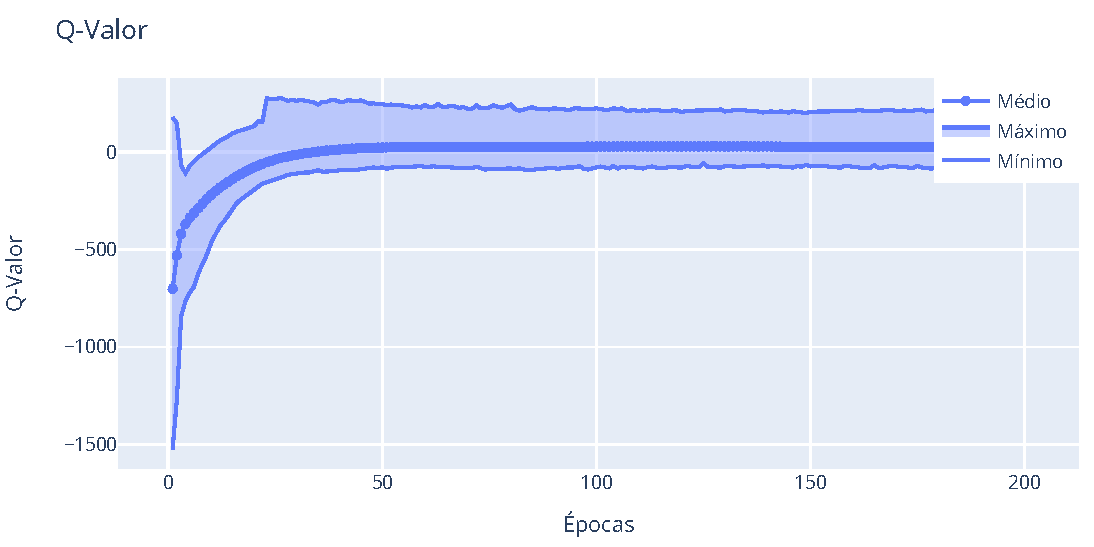
\includegraphics[width=\linewidth]{img/ddpg/petr3/clean/qval}
        \caption{PETR3 - Comportamento do QValor} 
        \label{ptr_clean_qval}
    \end{minipage}
    \quad
    \begin{minipage}[b]{0.45\linewidth}
        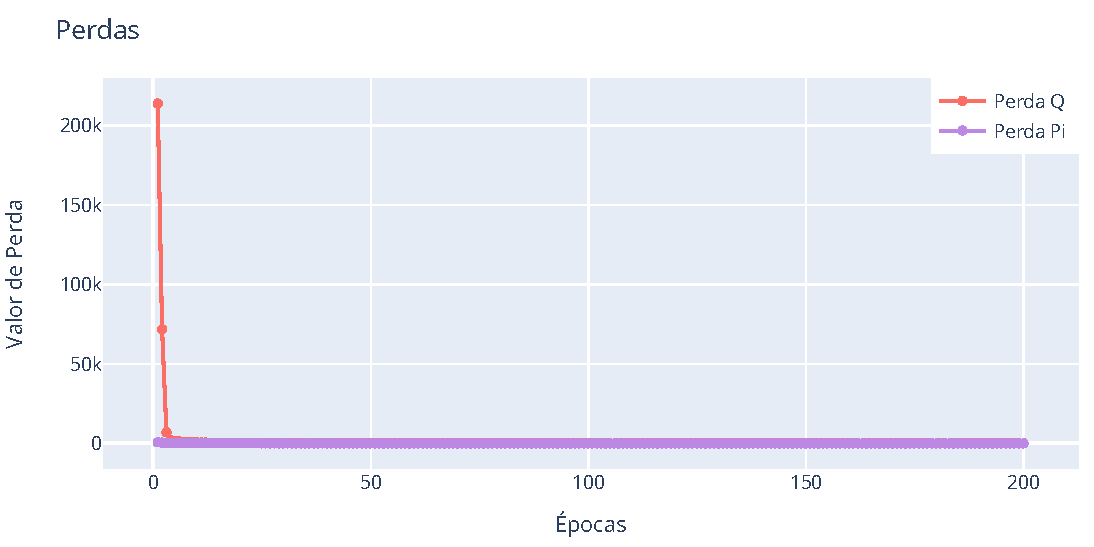
\includegraphics[width=\linewidth]{img/ddpg/petr3/clean/loss}
        \caption{PETR3 - Comportamento das funções de perda}
        \label{petr_clean_loss}
    \end{minipage}
\end{figure}

Em relação ao lucro obtido, nota-se na \refFig{petr_clean_ptrain}, que durante o treino se obteve uma alta dispersão de valores, fruto do alto ruido introduzido no treinamento, incluindo encontrar um lucro de $4670$ em um dos episódios. No entanto, o algoritmo não decide aproveitar o comportamento encontrado para esse lucro. 

\figura[htbp]{img/ddpg/petr3/clean/profit_train}{PETR3 - Lucro em treino}{petr_clean_ptrain}{width=.5\linewidth}

Quando o resultado do lucro é observado em teste (\refFig{petr_clean_profit}), percebe-se ainda as diversas oscilações apresentadas no treino, além de também não explorar a politica com maior lucro encontrada. O fato do algoritmo divergir de forma significativa e não explorar necessariamente o maior lucro pode estar relacionada com a formulação da função de recompensa, que não reflete exatamente o lucro obtido. No entanto, mesmo com essas variações presentes, o modelo obteve um lucro final médio em teste de R\$$1377,00$, realizando majoritariamente ações de compra (veja a \refFig{petr_clean_act}), quase não vendendo nem esperando. Vale enfatizar que nem toda ação de compra é realizada, se o agente não possui a quantidade de dinheiro para a compra ele recebe uma punição pela ação realizada de forma incorreta, o porquê do agente preferir uma punição a uma ação de espera é algo a ser explorado.

\begin{figure}[htbp]
    \centering 
    \begin{minipage}[b]{0.45\linewidth}
        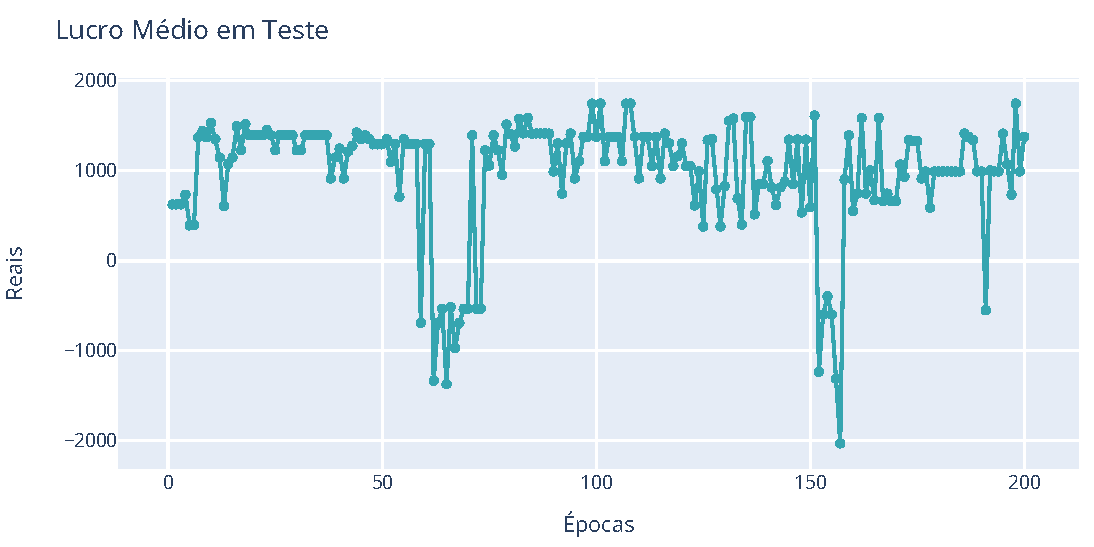
\includegraphics[width=\linewidth]{img/ddpg/petr3/clean/profit}
        \caption{PETR3 - Lucro médio em teste.} 
        \label{petr_clean_profit}
    \end{minipage}
    \quad
    \begin{minipage}[b]{0.45\linewidth}
        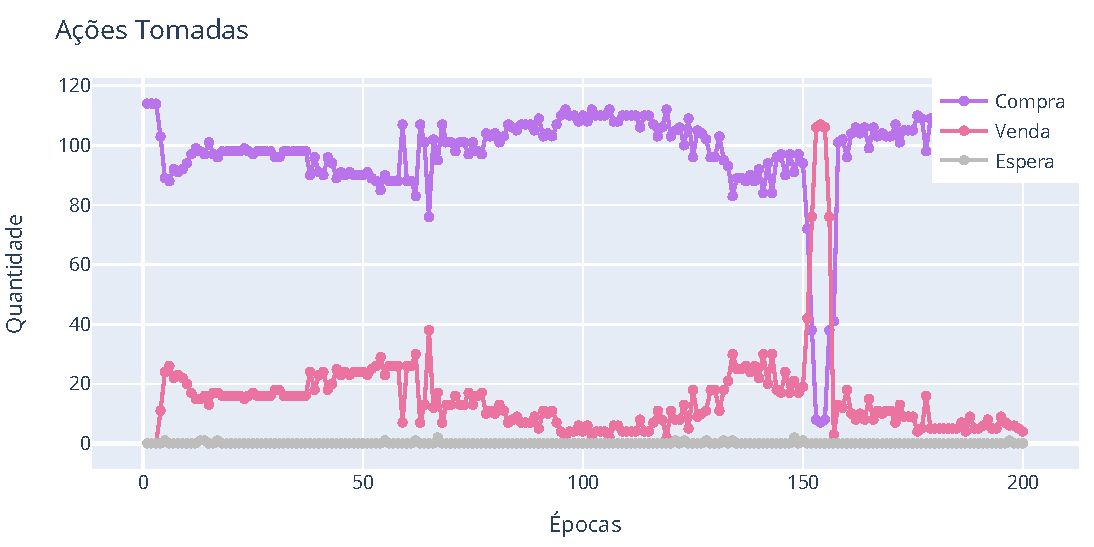
\includegraphics[width=\linewidth]{img/ddpg/petr3/clean/actions}
        \caption{PETR3 - Quantidade de ações selecionadas em teste.}
        \label{petr_clean_act}
    \end{minipage}
\end{figure}

Portanto, nota-se que o modelo, apesar de todas as adversidades encontradas, obteve um lucro de R\$$1377,00$ no final do teste, uma rentabilidade de $13,77\%$ no total dos 6 meses. A rentabilidade encontrada é $311,04\%$ maior que da poupança e $182,75\%$ maior que o \acrshort{CDI}. No caso de um investidor seguindo uma estratégia \emph{buy and hold}, o mesmo compraria o ativo a R\$$15,01$, com $10.000$ reais esse investidor compraria $600$ cotas a R\$$9.006$, e sobraria $994$ reais em conta. No fim do período, as ações da PETR3 estavam valendo R\$$16,05$, e portanto, o seu portfólio estaria valendo R\$$9.6300$, totalizando R\$$10.624$ com o dinheiro em conta, uma rentabilidade de $6,24\%$ no final do período. A estratégia de investimento aprendida pelo agente para operar no ativo, possui uma rentabilidade $120,67\%$ maior que o investidor seguindo um comportamento \emph{buy and hold}.
 
\subsection{Alocação do Ativo VALE3}

O segundo ativo individual a analisado foi o VALE3, Os experimentos realizados para este ativo possuem a mesma configuração de janela e de investimento inicial do ativo PETR3 previamente apresentado. As \refFigs{vale_clean_qval}{vale_clean_act}, demonstram todos os dados obtidos, também utilizando 200 épocas de treino e $10$ testes por época. Novamente realiza-se a análise começando pelo gráfico de retorno médio por episódios de treino e teste, demonstrados na \refFig{vale_clean_ret}. Diferentemente do ativo da PETR3, o retorno apresentado nas simulações da VALE não possuem tanta oscilação, indicando uma menor exploração pelo modelo. No final da simulação, o algoritmo obtém um retorno médio de $-3.327$ para ambos treino e teste, mesmo tendo encontrado um retorno de $31,83$ ao longo de sua trajetória. 

\figura{img/ddpg/vale3/clean/return}{VALE3 - Retorno médio}{vale_clean_ret}{width=.5\linewidth}

De forma similar ao ativo anterior, analisa-se também as \refFigs{vale_clean_qval}{vale_clean_loss} para entender o comportamento do Q-Valor médio e das funções de perda. O Q-Valor obtido possui uma média de $-11.31$, variando entre $51.44$ e $-135.28$. Tal valor médio negativo de Q-Valor, junto com um mínimo tão discrepante da média justificam o retorno negativo médio obtido pelo modelo. Por outro lado, as funções de perda assumem os valores mais próximos de $0$, com $21.13$ para a aproximação do Q-Valor e $11.18$ para aproximação da política, o que pode ser um indicativo de que este modelo é mais adaptável a replicações em relação ao do ativo PETR3. 

\begin{figure}[htbp]
    \centering 
    \begin{minipage}[b]{0.45\linewidth}
        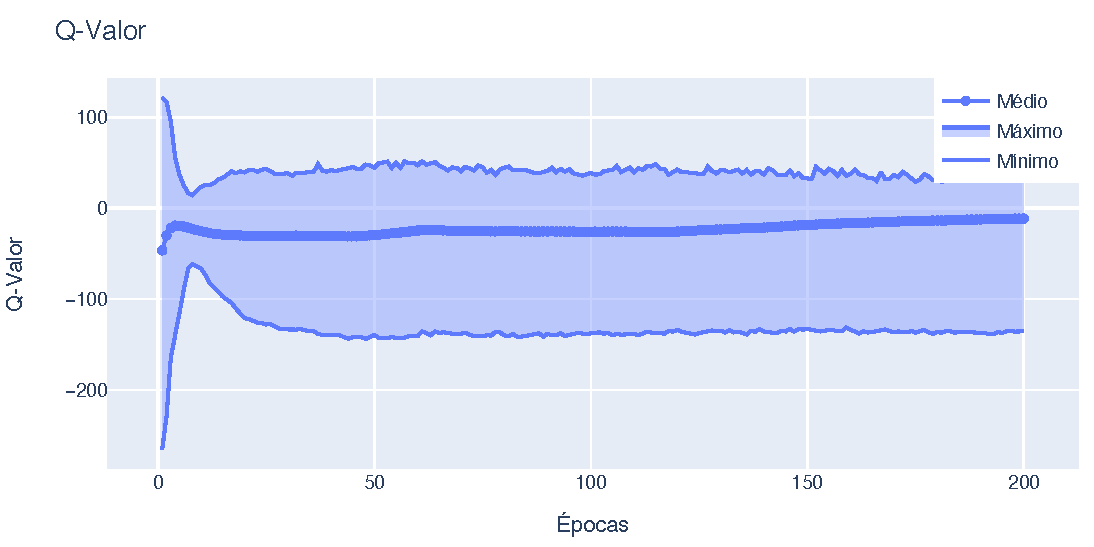
\includegraphics[width=\linewidth]{img/ddpg/vale3/clean/qval}
        \caption{VALE3 - Comportamento do QValor.} 
        \label{vale_clean_qval}
    \end{minipage}
    \quad
    \begin{minipage}[b]{0.45\linewidth}
        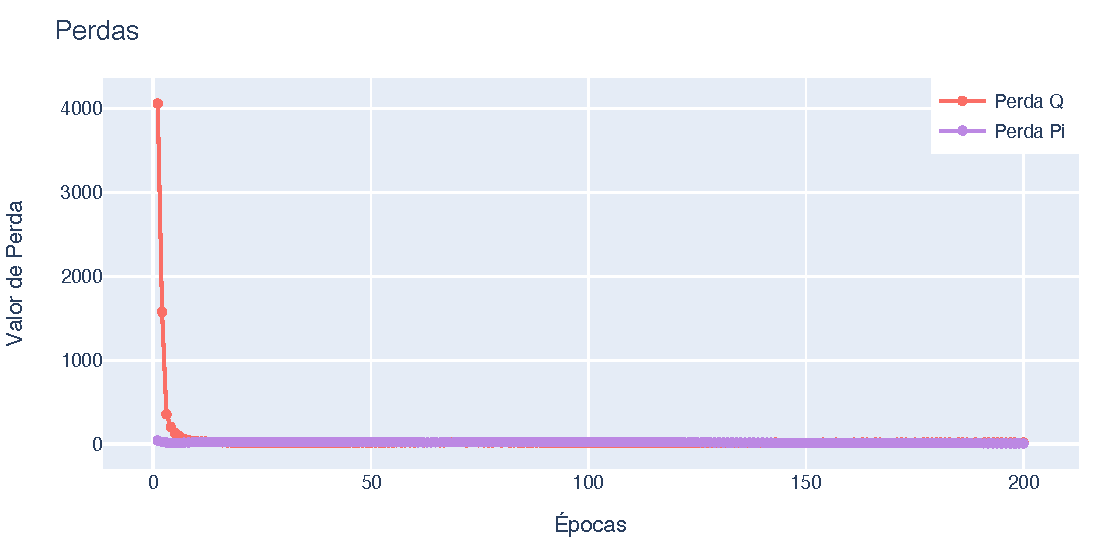
\includegraphics[width=\linewidth]{img/ddpg/vale3/clean/loss}
        \caption{VALE3 - Comportamento das funções de perda.}
        \label{vale_clean_loss}
    \end{minipage}
\end{figure}

Com base no lucro obtido durante a fase de treino, apresentado na \refFig{vale_clean_ptrain}, nota-se também uma alta dispersão dos valores chegando a encontrar lucros maiores que mil reais, mas esses não foram explorados. Observa-se que a conversão para um valor de lucro constante acontece bem mais rápido, e mesmo com o ruido presente, o treino não varia a mesma quantidade de PETR3.

\figura[htbp]{img/ddpg/vale3/clean/profit_train}{VALE3 - Lucro em treino}{vale_clean_ptrain}{width=.5\linewidth}

Quando o valor do lucro é analisado em teste (\refFig{vale_clean_profit}), percebe-se um padrão similar a média de lucro obtida no treino. O maior lucro encontrado durante a simulação foi de R\$$942,00$, no entanto, o valor final para qual o algoritmo converge é de apenas $603,00$ reais. Este comportamento reforça a hipótese de que a função de recompensa pode ser responsável pela falta de aproveitamento do agente por lucros maiores. Em relação as ações, apresentadas na \refFig{vale_clean_act}, o comportamento selecionado é discrepante com o realizado para o ativo da PETR3, realizando majoritariamente ações de venda, quase não vendendo e nunca esperando. De forma similar, enfatiza-se que nem toda ação de venda é realizada, se o agente não possui ativos para vender ele recebe uma punição pela ação realizada de forma incorreta. Também é incerto o porquê do agente não aproveitar os comportamentos de espera.

\begin{figure}[htbp]
    \centering 
    \begin{minipage}[b]{0.45\linewidth}
        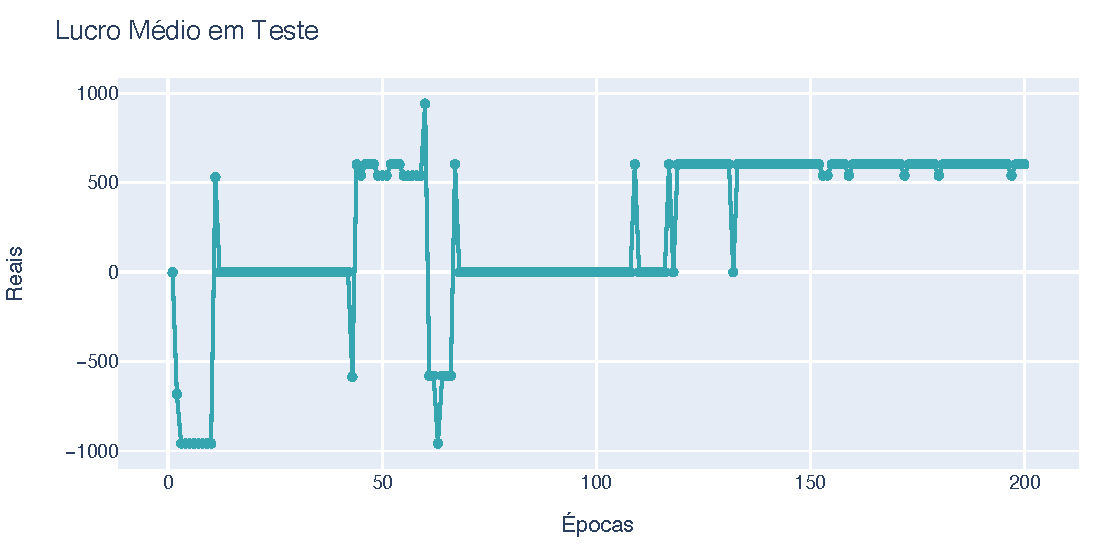
\includegraphics[width=\linewidth]{img/ddpg/vale3/clean/profit}
        \caption{VALE3 - Lucro médio em teste.} 
        \label{vale_clean_profit}
    \end{minipage}
    \quad
    \begin{minipage}[b]{0.45\linewidth}
        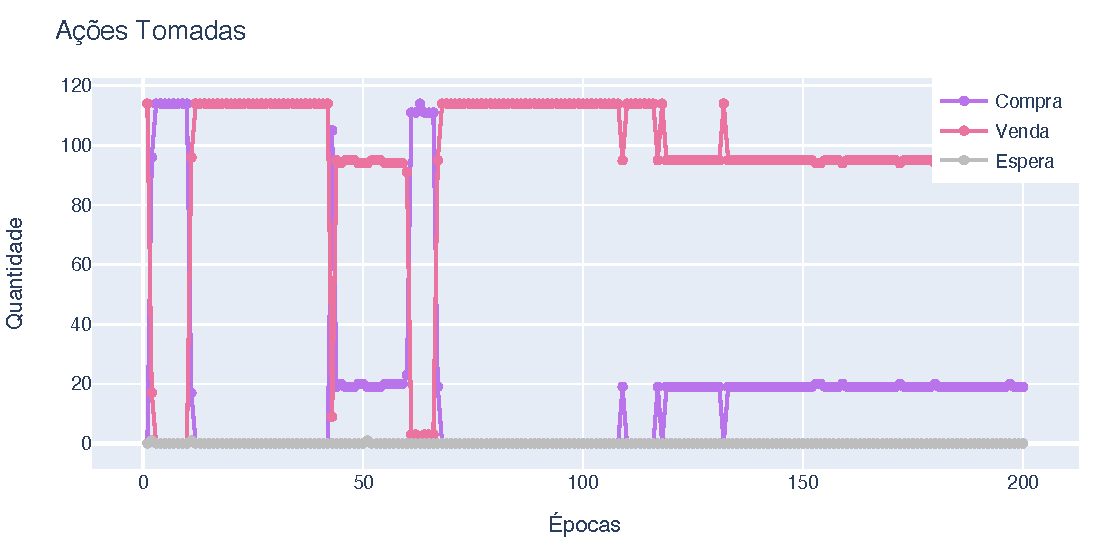
\includegraphics[width=\linewidth]{img/ddpg/vale3/clean/actions}
        \caption{VALE3 - Quantidade de ações selecionadas em teste.}
        \label{vale_clean_act}
    \end{minipage}
\end{figure}

Analisando o desempenho do modelo, percebe-se que as adversidades impactaram de forma significante a capacidade do agente lucrar, obtendo um lucro de apenas R\$$603,00$. Este lucro representa uma rentabilidade de $6,03\%$ no total dos 6 meses. No entanto, a rentabilidade, apesar de baixa, ainda oferece lucratividade $80\%$ e $23,81\%$ maior que a poupança e o CDI respectivamente. Considerando a estratégia \emph{buy and hold} de um investidor, os ativos da VALE3 seriam comprados inicialmente pelo valor de R\$$32,25$, o que permitira a compra de $300$ cotas a R\$$9.675$ e sobraria R\$$325$ em conta. No fim do período estipulado para a simulações, as ações da VALE3 alcançariam um valor de R\$$29.06$. O investidor que tivesse alocado essa quantia nos ativos da Vale nesse período perderia $957$ reais, terminando com $8.718$ em ativos, totalizando com o saldo em carteira $9.043$, uma rentabilidade de $-9,57\%$. A estratégia de investimento aprendida pelo agente, apesar de não apresentar grandes lucros, demonstra uma aversão a perdas, sabendo parar de investir quando algum lucro foi obtido.


\subsection{Alocação do Ativo ABEV3}

Finalizando, o ultimo ativo individual a ser analisado foi o ABEV3. Neste ativo também foi utilizado R\$$10.000$ de valor inicial, mas diferentemente da PETR3 e VALE3, a janela utilizada foi de 9 dias, similar ao resultado da \acrshort{LSTM}. Os dados obtidos nos experimentos estão representados nas \refFigs{abev_clean_ret}{abev_clean_act}, onde cada experimento também acontece em $200$ épocas de treino e $10$ episódios de teste por época. A \refFig{vale_clean_ret}, apresenta o retorno médio por episódios de treino e teste. Para o ativo especifico da ABEV3, o modelo não conseguiu generalizar a ponto de obter lucros. Acredita-se que este comportamento pode ser fruto da dificuldade do agente em encontrar recompensas positivas significantes no começo da simulação, entrando em uma situação de \emph{deadlock}, onde o algoritmo da \acrshort{DDPG} falha em aprender \cite{}. No final da simulação, o algoritmo obtém um retorno médio de $-61.05$ para treino e $-68.70$ para teste, mesmo tendo encontrado retornos maiores ao longo de sua trajetória. 

\figura{img/ddpg/abev3/clean/return}{ABEV3 - Retorno médio}{abev_clean_ret}{width=.5\linewidth}

A busca pelo entendimento desse comportamento para o ativo da ABEV3, segue com a análise das \refFigs{abev_clean_qval}{abev_clean_loss}. Essa análise busca entender o comportamento do Q-Valor médio e das funções de perda, que levaram a um desempenho ruim. O Q-Valor obtido possui uma média de $-27.59$, variando entre $98.05$ e $-154.09$. Em relação as função de perda, aproximação do Q-Valor chega a $13.59$, enquanto a aproximação de $\pi$ a ultrapassa, chegando a $27.57$, claramente divergindo da politica buscada.

\begin{figure}[htbp]
    \centering 
    \begin{minipage}[b]{0.45\linewidth}
        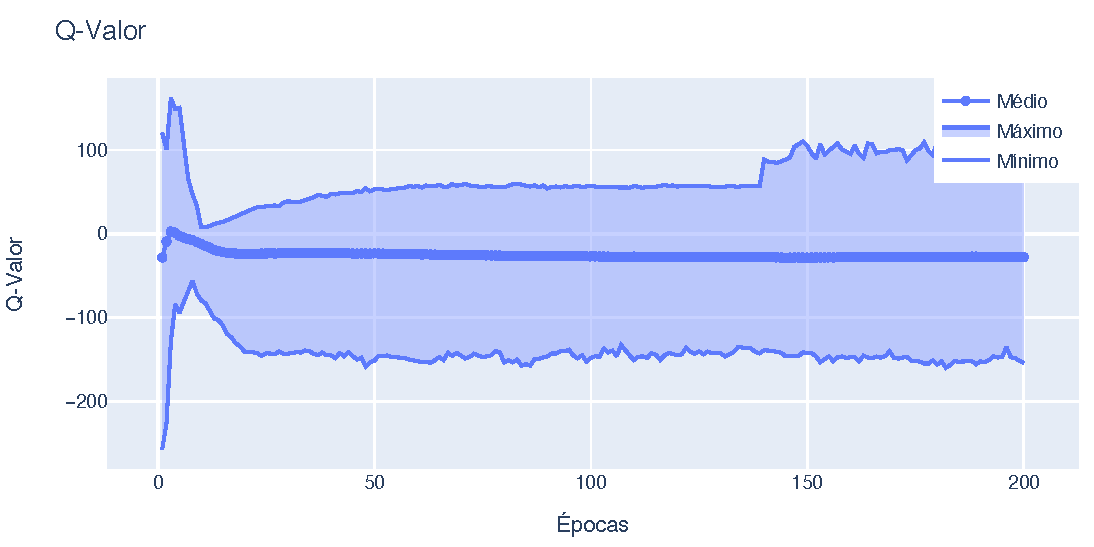
\includegraphics[width=\linewidth]{img/ddpg/abev3/clean/qval}
        \caption{ABEV3 - Comportamento do QValor.} 
        \label{abev_clean_qval}
    \end{minipage}
    \quad
    \begin{minipage}[b]{0.45\linewidth}
        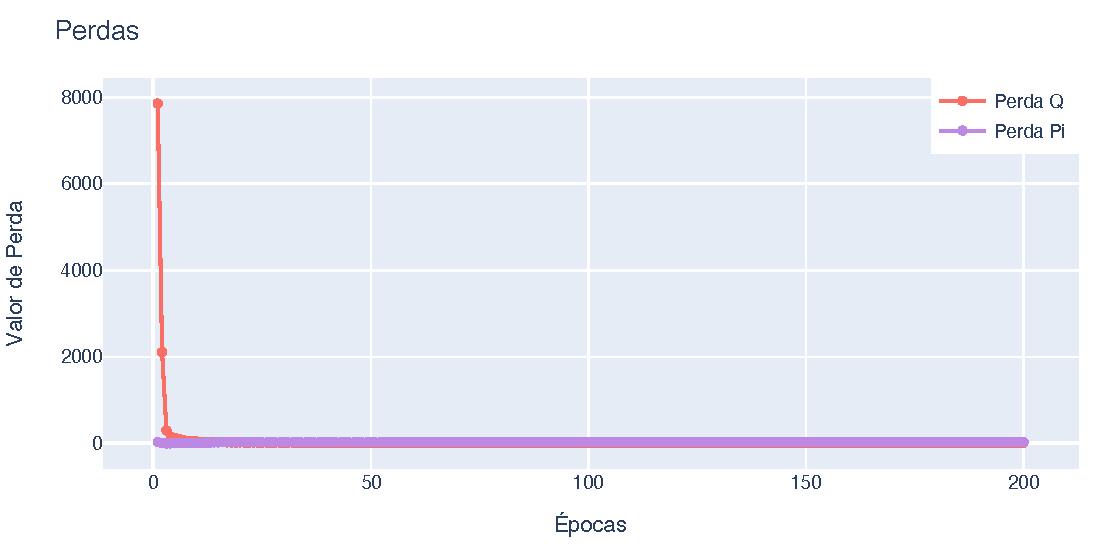
\includegraphics[width=\linewidth]{img/ddpg/abev3/clean/loss}
        \caption{ABEV3 - Comportamento das funções de perda.}
        \label{abev_clean_loss}
    \end{minipage}
\end{figure}

Nota-se na \refFig{abev_clean_ptrain}, que o lucro médio obtido durante a fase de treino, fica sempre perto de zero, mesmo apresentando dispersões de mil reais para mais ou para menos. Observa-se que a conversão para um valor de lucro constante não acontece de forma aparente, o que pode ser apenas o ruido presente nas ações, mas pode ser um indicio de que o algoritmo entrou em seu estado de \emph{deadlock}.

\figura[htbp]{img/ddpg/abev3/clean/profit_train}{ABEV3 - Lucro em treino}{abev_clean_ptrain}{width=.5\linewidth}

Quando o valor do lucro é analisado em teste (\refFig{abev_clean_profit}), percebe-se que a politica de aversão a perdas, vista no ativo da VALE3 também foi aprendida. O agente termina a simulação com um nenhum lucro, mas também nenhuma perda, exatamente $0$, mesmo eventualmente o agente encontrando alguns lucros baixos de R\$$140,00$. Novamente, esse comportamento impede o aproveitamento do agente por lucros maiores, o que pode ser causado pela função de recompensa. Em relação as ações, apresentadas na \refFig{abev_clean_act}, o comportamento selecionado apresenta claramente o lucro de $0$, visto que o agente decide só vender desde o inicio da simulação, se avergindo a investir. Observe também que quando o agente tentou explorar as outras ações o agente obteve perdas significantemente maiores que ganhos, o que pode ter causado uma espécie de desistência pelo lado do agente. 

\begin{figure}[htbp]
    \centering 
    \begin{minipage}[b]{0.45\linewidth}
        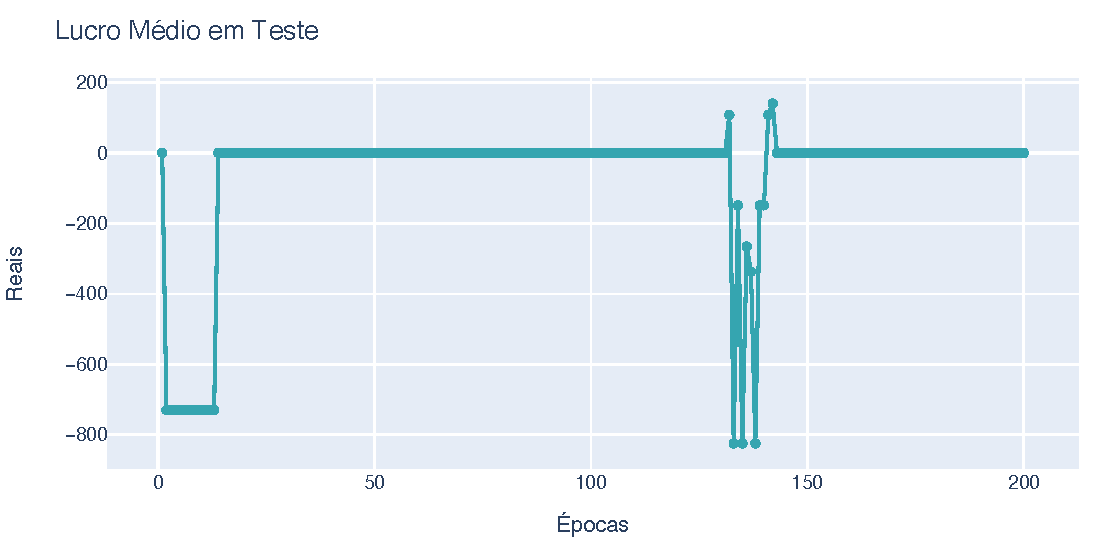
\includegraphics[width=\linewidth]{img/ddpg/abev3/clean/profit}
        \caption{ABEV3 - Lucro médio em teste.} 
        \label{abev_clean_profit}
    \end{minipage}
    \quad
    \begin{minipage}[b]{0.45\linewidth}
        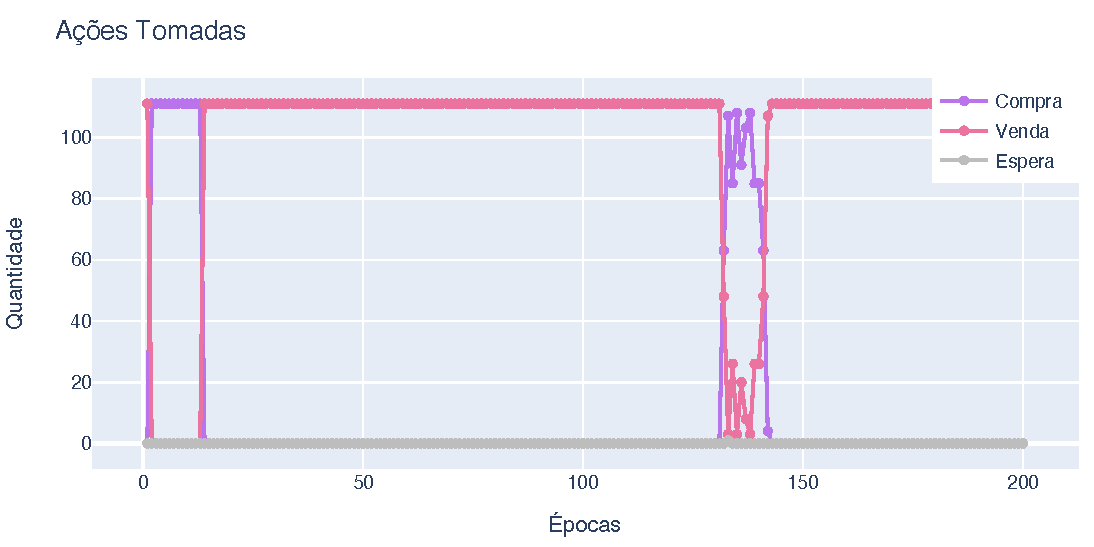
\includegraphics[width=\linewidth]{img/ddpg/abev3/clean/actions}
        \caption{ABEV3 - Quantidade de ações selecionadas em teste.}
        \label{abev_clean_act}
    \end{minipage}
\end{figure}

O desempenho do modelo para o ativo ABEV3 não é o esperado, no entanto, ainda assim o modelo evita a possibilidade de perdas. Este ativo, no inicio do período de investimento, estava sendo vendido a $17$ reais, mas no fim do período, o ativo chegaria a $15.54$, desvalorizando em $9,3\%$. Um investidor seguindo a estratégia \emph{buy and hold} possuiria grandes perdas nesse ativo. O que confirma mais uma vez, que a estratégia aprendida pelo agente, apesar de não ser ótima, consegue evitar prejuízos ao investidor.

\subsection{Alocação do Portfólio Completo}

No entanto, todos os experimentos analisados até o momento utilizam apenas um ativo específico, uma contradição a Teoria Moderna do Portfólio, que diz que os fatores devem ser calculados e analisados em relação ao conjunto de ativos \cite{markowitz}. Esse experimento busca então analisar o desempenho do agente com um portfólio diversificado de ativos. O portfólio foi então construído com os ativos utilizados nos experimentos anteriores (PETR3, VALE3 e ABEV3) e suas janelas respectivas. Com o propósito de aumentar a quantidade de ativos que o agente consegue investir, a quantidade de dinheiro inicial foi definida como R\$$50.000$. As \refFigs{all_clean_qval}{all_clean_act}, demonstram os dados obtidos em 200 épocas de experimentos. A \refFig{all_clean_qval} apresenta o comportamento do retorno médio obtido por episódios de treino e teste. Observe que diferente dos ativos individuais o retorno chega a assumir valores bem maiores, resultado consequente da maior quantidade de recursos inserida no sistema. Nota-se também que é visível a convergência do retorno médio de treinamento ao longo do treino e teste, obtendo um valor final de $404.24$ para ambos treino e teste.

\figura{img/ddpg/all/clean/return}{Portfólio - Retorno médio}{all_clean_ret}{width=.5\linewidth}

Analisa-se também o Q-Valor médio e as funções de perda do treinamento, com base nas \refFigs{ptr_clean_qval}{petr_clean_loss}. O Q-Valor alcança uma média de $230,84$, variando entre $1633,95$ a $-594,62$, enquanto as funções de perda assumem valores de $2.357,02$ e $-232.13$ para perda Q (função de aproximação do Q-Valor) e perda $\pi$ (função de aproximação da politica) respectivamente. Nota-se que os valores de perda são maiores que dos ativos individuais, o que representa uma correlação entre a recompensa maior obtida, devido a maior quantidade de recursos no sistema. Apesar desses valores ainda serem extremamente altos para funções de perda, experimentos com maiores números de época não apresentaram resultados diferentes ao comportamento.

\begin{figure}[htbp]
    \centering 
    \begin{minipage}[b]{0.45\linewidth}
        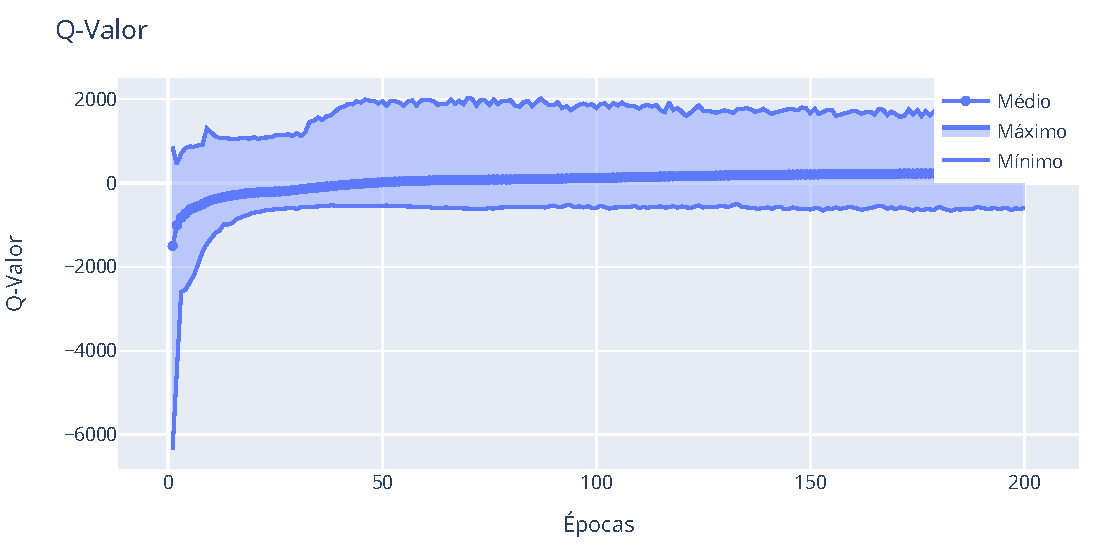
\includegraphics[width=\linewidth]{img/ddpg/all/clean/qval}
        \caption{Portfólio - Comportamento do QValor.} 
        \label{all_clean_qval}
    \end{minipage}
    \quad
    \begin{minipage}[b]{0.45\linewidth}
        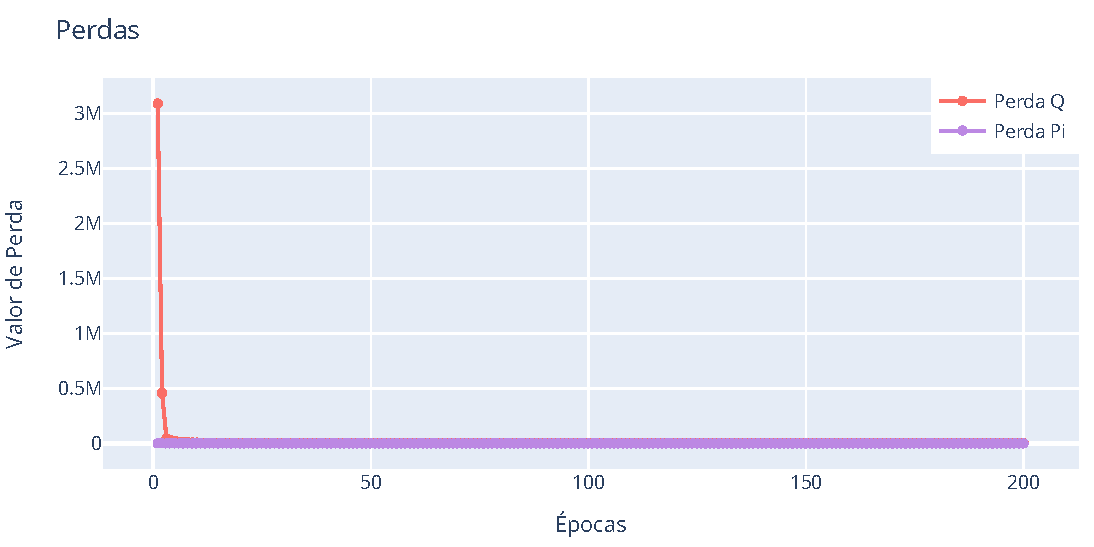
\includegraphics[width=\linewidth]{img/ddpg/all/clean/loss}
        \caption{Portfólio - Comportamento das funções de perda.}
        \label{all_clean_loss}
    \end{minipage}
\end{figure}

Em relação ao lucro obtido, nota-se na \refFig{all_clean_ptrain}, que durante o treino se obteve uma alta dispersão de valores, incluindo um lucro de R\$$23.860$ em um dos episódios. Novamente, no entanto, o algoritmo não explora essas recompensas maiores. Esse comportamento também foi observado nos outros experimentos, o estudo do mesmo abre possibilidades para trabalhos futuros que podem ser capazes de melhorar significantemente os modelos. Se o agente tivesse explorado o melhor lucro encontrado, teria obtido um rendimento de aproximadamente $47\%$ no período, quase $8\%$ ao mês.  

\figura[htbp]{img/ddpg/all/clean/profit_train}{Portfólio - Lucro em treino}{all_clean_ptrain}{width=.5\linewidth}

Quando o resultado do lucro é observado em teste (\refFig{petr_clean_profit}), percebe-se oscilações menores (por não conter ruido em suas ações), e nota-se que também não é explorada a politica com maior lucro encontrada. No entanto, mesmo com essas limitações presentes no modelo proposto, ao final do treinamento obteve-se um lucro médio de $5.874$ reais, realizando ações majoritariamente de venda, comprando algumas vezes, e nunca realizando a ação de espera (veja a \refFig{all_clean_act}). Observa-se que a ação de espera raramente é selecionada em experimentos, sendo de ativos individuais ou do portfólio completo, esse comportamento provavelmente é fruto da função de recompensa, cabendo a trabalhos futuros investigar como adaptar a função para melhorar o sistema.

\begin{figure}[htbp]
    \centering 
    \begin{minipage}[b]{0.45\linewidth}
        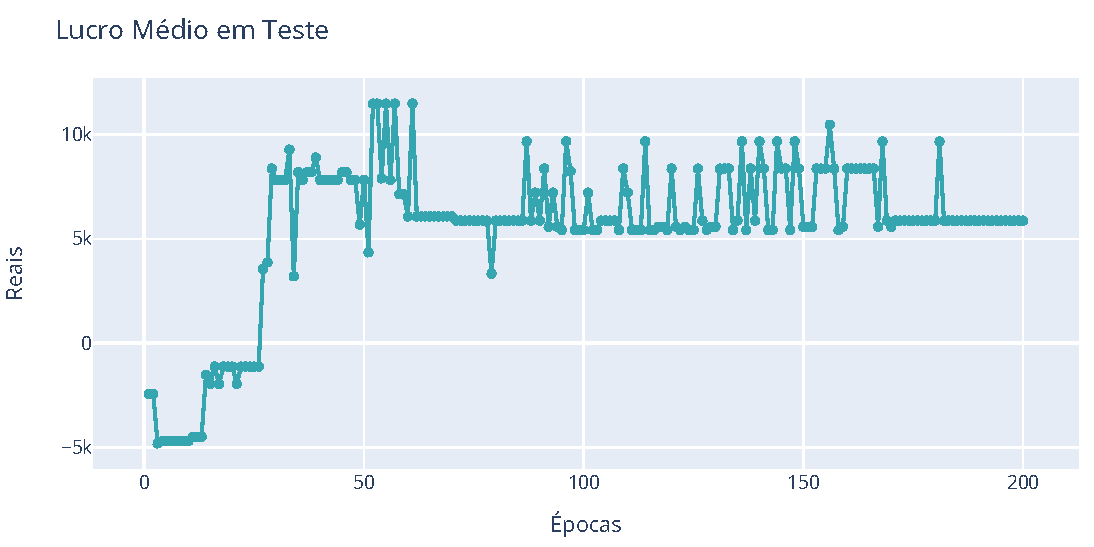
\includegraphics[width=\linewidth]{img/ddpg/all/clean/profit}
        \caption{Portfólio - Lucro médio em teste.} 
        \label{all_clean_profit}
    \end{minipage}
    \quad
    \begin{minipage}[b]{0.45\linewidth}
        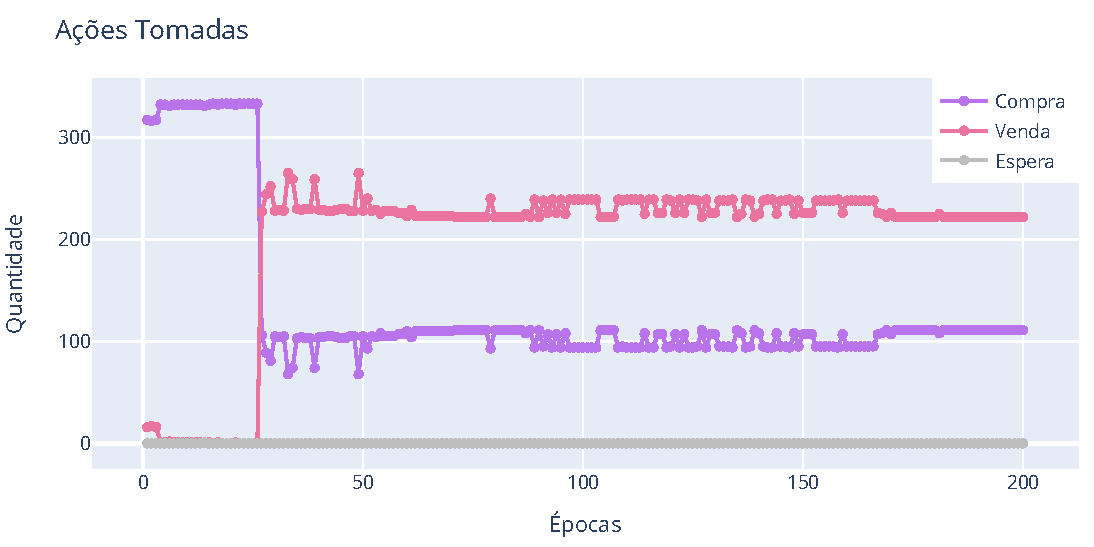
\includegraphics[width=\linewidth]{img/ddpg/all/clean/actions}
        \caption{Portfólio - Quantidade de ações selecionadas em teste.}
        \label{all_clean_act}
    \end{minipage}
\end{figure}

Portanto, nota-se que o modelo, apesar de todas as adversidades encontradas, obteve um lucro de R\$$5.874,00$ no final do teste, uma rentabilidade de $11,74\%$ no total dos 6 meses. A rentabilidade encontrada é $250,44\%$ maior que da poupança e $141,06\%$ maior que o \acrshort{CDI}. Nota-se que a rentabilidade encontrada é um pouco menor que a rentabilidade do ativo PETR3. Essa diferença pode ser justificada pelo fato do ativo da Petrobras ser o único que valoriza no período avaliado, sendo possível que o modelo entenda o risco de investir nos outros ativos.

A análise do investidor seguindo uma estratégia \emph{buy and hold}, para essa situação demanda um estudo um pouco mais complicado. Essa complicação é devido ao fato de existir infinitas maneiras no qual um investidor pode montar seu portfólio com três ativos. Para o propósito desse trabalho, o construiu-se um portfólio comparativo considerado ótimo, seguindo a teoria de Markowitz. O processo em construção desse portfólio leva em consideração a quantificação do retorno e o risco individual de cada ativo para posteriormente achar uma fronteira eficiente que tenha a maior possibilidade de retorno para a quantidade de risco que se deseja assumir.

\subsubsection{Análise Comparativa Com Fronteira Eficiente}

A \refFig{fronteira_port} apresenta diversas combinações de portfólios existentes em relação ao retorno esperado para o primeiro semestre de $2014$ e o risco assumido pelo mesmo. Para calcular esses valores, é utilizado como base os preços de fechamento mensais ajustado de cada ativo\footnote{Dados retirados do site: \url{http://finance.yahoo.com}}, de $2011$ a $2013$. Com os preços, calcula-se então os retornos e riscos mensais, informações utilizadas para compor a carteira. A cor de cada combinação de portfólio é respectiva a um indicador que ajuda a descobrir um ponto de equilíbrio entre risco e retorno, denominado Índice de Sharpe. Esse indicador mede o retorno excedente de uma aplicação financeira em relação a outra aplicação livre de risco. A aplicação livre de risco escolhida para calcular o índice, foi o retorno do \acrshort{CDI} no ano de $2013$ ($8,06\%$)\footnote{Dados retirados do site: \url{https://www.tororadar.com.br/}}, ano anterior ao que queremos estudar. 

\figura{img/fronteira}{Fronteira eficiente do portfólio PETR3, VALE3, ABEV3}{fronteira_port}{width=\linewidth}

Os diversos portfólios que foram gerados na \refFig{fronteira_port} são frutos da aplicação de um método que tem como objetivo gerar simulações aleatórias de forma massiva para encontrar um resultado aproximado da realidade, denominado método de Monte Carlo. A fronteira eficiente foi então encontrada com um conjunto de $25.000$ simulações aleatórias. Dentro da fronteira, qualquer portfólio selecionado será considerado ótimo (de maior retorno e menor risco). No entanto, para esse trabalho consideramos dois portfólios apenas, o de menor risco, e o de maior índice de Sharpe, representados respectivamente pelos marcadores verde e vermelho. A carteira de menor risco estima um retorno semestral de $1.18\%$, com um risco de $45\%$, sendo construída de $17.86\%$ PETR3, $42.91\%$ VALE3 e $39.22\%$ ABEV3. Por outro lado, a carteira de maior índice de Sharpe, possui um potencial de retorno de $4.28\%$ com um risco de $80\%$, sendo construída por $4.54\%$ PETR3, $0.1\%$ VALE3 e $95.36$ ABEV3.

Tendo a porcentagem de cada ativo para cada portfólio podemos então criar os portfólios em que um investidor alocaria seu saldo de R\$$50.000$. Começando pela estratégia mais segura, seguindo o portfólio de menor risco, o investidor distribuiria seu dinheiro nos ativos da forma supracitada. Relembrando, os preços iniciais dos ativos no período inicial de 2014 são $15,01$ para PETR3, $32,25$ para VALE3 e $17,00$ para ABEV3. Nesses valores, o portfólio de menor risco, com os pesos resultantes da fronteira eficiente, consistiria de $500$ cotas da PETR3, $600$ cotas da VALE3 e $1100$ cotas da ABEV3, totalizando R\$$45.555$ investidos, e sobrando R\$$4.445$\footnote{Os valores selecionados para as quantidades de cotas são calculados com base na porcentagem de dinheiro que deve ser investido naquele ativo. Neste trabalho, consideramos que o agente não pode comprar ações fracionadas, apenas em lotes, portanto, a quantidade de cotas é sempre arredondada para a centena inferior.}. Os valores finais assumidos pelos ativos, no período analisado, foram de $16,05$ para PETR3, $29,06$ para VALE3 e $15,54$ para ABEV3. Desta forma o investidor que segui-se o portfólio de menor risco obteria um lucro de $520$ na Petrobras, mas perderia $1.914$ com a Vale e $1.606$ com a Ambev. Obtendo um rendimento total de $-3000$ reais do valor investindo e totalizando sua carteira com $47.000$ reais. O investidor que escolhesse pelo portfólio com maior índice de Sharpe seguiria por um caminho similar. Sua carteira seria alocada de $100$ cotas da PETR3, $0$ cotas da VALE3 e $2800$ cotas da ABEV3, totalizando R\$$49.101$ investidos, e sobrando R\$$899$ de saldo. Este investidor ganharia $104$ reais na Petrobras, $0$ na Vale, e seria abatido por uma perda de $-4.088$ reais. O mesmo perderia R\$$3.984$ do dinheiro investido, totalizando $46.016$ reais na carteira.

O primeiro semestre de 2014 não viria a ser um período lucrativo para um investidor que seguisse o modelos de composição de portfólio baseados na fronteira eficiente. Os portfólios de menor risco e maior índice de Sharpe que possuíam capacidades para apresentar retornos de $1,18\%$ e $4,28\%$, sucumbiram a seus riscos, fornecendo uma rentabilidade real de $-6\%$ e $-7,96\%$. Portanto, o investidor que seguisse o modelo treinado com o \acrshort{DDPG} proposto pelo Hare, obteria no final dos 
$6$ meses uma rentabilidade de $11,74\%$, um retorno claramente maior que os retornos reais e projetados dos portfólios considerados ``eficientes''. Demonstrando assim, a viabilidade do modelo proposto para investimentos na bolsa de valores.

\subsubsection{Experimento Extra com o Módulo de Gerenciamento de Riscos}

Após todos os experimentos analisados com os estados preditivos dos ativos, realizou-se então um novo experimento com informações de riscos fornecidas pelo módulo de gerenciamento de risco sintético implementado. O experimentos foram realizados com parâmetros similares ao experimento de portfólio previamente realizado. Sua única diferença foi em relação ao estado do agente, agora o agente além de ter acesso a predição do ativo, tem acesso também ao indicador de riscos do \acrshort{MGR}.

Para cada ativo do portfólio, utiliza-se o volume de consultas do mesmo no \emph{Google Trends}. Esse volume representa a quantidade de pesquisas semanais entre $0$ a $100$ do termo pesquisado. No entanto, o \acrshort{MGR} processa essa informação, indicando um risco com o valor $1$ caso o valor esteja acima de um limite pré-determinado, ou $0$ caso o contrário. O experimento realizado possui um valor limite de $90$, representando que apenas pesquisas demasiadas indicariam um risco.

As \refFigs{all_risk_profit}{all_risk_act}, apresentam os resultados para o experimento. Como podemos ver, o experimento apresenta resultados semelhantes ao anterior (sem o \acrshort{MGR}). No entanto apresenta menos variações em seus resultados de teste em relação os valores encontrados sem o risco. O lucro encontrado é idêntico ao do experimento anterior, R\$$5.874,00$ no final do teste, uma rentabilidade de $11,74\%$ no total dos 6 meses. Sendo a única diferença aparente a impressão de uma conversão mais rápida ao resultado encontrado. Os outros gráficos obtidos durante o experimento foram omitidos por possuírem resultados muito similares ao experimento anterior. 

\begin{figure}[htbp]
    \centering 
    \begin{minipage}[b]{0.45\linewidth}
        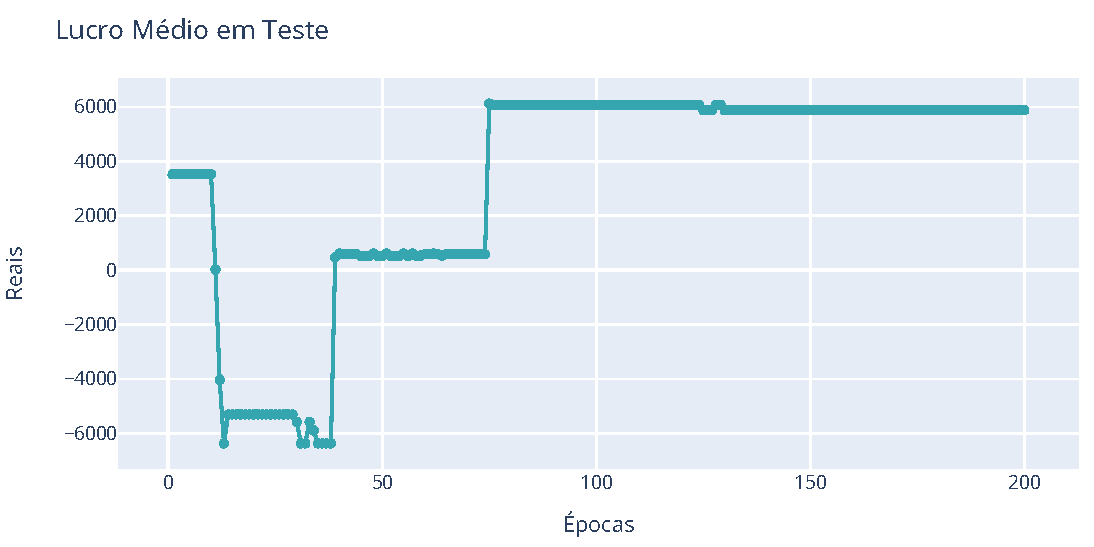
\includegraphics[width=\linewidth]{img/ddpg/all/risk/profit_test.pdf}
        \caption{Portfólio com \acrshort{MGR} - Lucro médio em teste.} 
        \label{all_risk_profit}
    \end{minipage}
    \quad
    \begin{minipage}[b]{0.45\linewidth}
        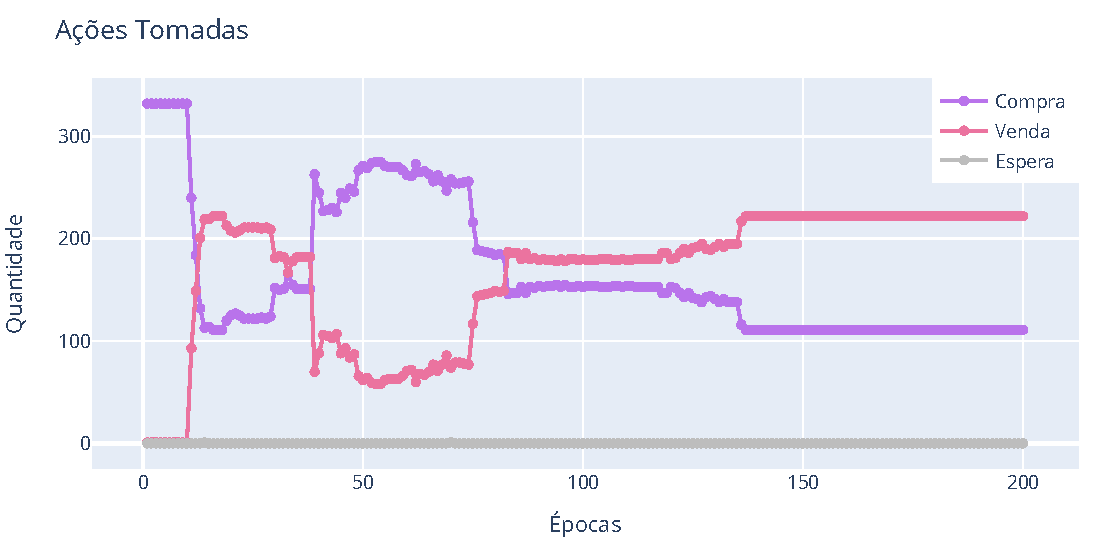
\includegraphics[width=\linewidth]{img/ddpg/all/risk/actions.pdf}
        \caption{Portfólio com \acrshort{MGR} - Quantidade de ações selecionadas.}
        \label{all_risk_act}
    \end{minipage}
\end{figure}

A semelhança dos resultados encontrados pode ser um indicativo de que o módulo de risco sintético não apresenta consistência em sua informação, e seguindo essa lógica de raciocínio, invalidaria a premissa de que um alto numero de pesquisas representa necessariamente um risco. A implementação de modelos robustos para o \acrshort{MGR} e a análise mais profunda de seu comportamento será investigada em trabalhos futuros.

Com esses experimentos finaliza-se a análise do Módulo Alocador de Recursos, demonstrando sua eficiência e capacidade de gerar lucros investindo de forma autônoma. 

\section{Considerações Finais}
\label{exp:consideracoes}

Este capitulo realizou a validação do serviço proposto em duas etapas, primeiro validando o módulo preditor. seguindo com validação o \acrshort{MAR}. Validou-se o módulo preditor de forma individual para cada ativo, seguindo uma sequência de passos bem definidos. Criou-se uma rotina de exploração de hiper-parâmetros, realizou-se analises post-hoc nos resultados obtidos, e treinou-se os modelos que obtiveram os melhores desempenho. Os dados obtidos demonstraram resultados satisfatórios para os modelos criados, com acurácia de até $92.0\%$ no ativo PETR3, $82\%$ em VALE3, e $94\%$ em ABEV. Tais resultados foram comparados, avaliando o desempenho em relação a modelos de base selecionados da literatura. O modelo proposto obteve a maior acurácia e a maior média das métricas obtidas. Posteriormente, realizou-se a validação do \acrshort{MAR}, começando pelos ativos individuais até chegar no portfólio completo. Os resultados obtidos, mostraram uma rentabilidade de $13,77\%$ em PETR3, $6,03\%$ em VALE3, $0\%$ em ABEV, e $11,74\%$ para o portfólio completo. O resultado do portfólio foi comparado com um 
``portfólio eficiente'' criado utilizando a \acrshort{VMM}, obtendo resultados consideravelmente melhores, visto que o ``portfólio eficiente'' apresentaria perdas no fim do período analisado.
 
Os experimentos realizados no algoritmo \acrshort{DDPG} envolveram muitas tentativas (e erros), nos quais não foram mencionados. Diversas funções de recompensas foram testadas, estas incluem: valores simples como $-1$ e $+1$ para recompensas de perda ou lucro respectivamente, valores de recompensa somente no fim da simulação, recompensas baseadas em ganho diário, dentre diversas outras. Nenhuma das recompensas apresentou um resultado tão eficiente quanto o demonstrado, muita das vezes convergindo para uma politica especifica na primeira época e não explorando. Acredita-se que a \acrshort{DDPG} possa estar apresentando dois principais problemas à formulação da função recompensa: recompensas esparsas e falta de reforços positivos. Esses dois casos podem estar levando a \acrshort{DDPG} a uma situação de \emph{deadlock}, onde não consegue mais aprender \cite{}. Além das funções de recompensa, espaço de estados diversos também foram implementados, variando de todas as possíveis formas o espaço de estados apresentados no desenvolvimento, incluindo situações onde o espaço de estados possuía somente o indicador de movimento. Nenhum dos quais apresentaram resultados demonstráveis. Ademais, notou-se que a \acrshort{DDPG} é extremamente sensível a hyper-parametrização, desde a semente aleatória que gerará o modelo até o tamanho da camada escondida, diversos parâmetros foram testados, os apresentados nesse trabalho foram o obtiveram melhores resultados.

Portanto, ainda há muito a ser feito na validação do Hare para trabalhos futuros. Alguns pontos consideráveis de melhoria que poderiam ser realizados, envolvem: utilização de mais valores de entrada para o modelo \acrshort{LSTM}, criação de um modelo inteligente para o \acrshort{MGR}, hiper-parametrização da \acrshort{DDPG} utilizando o Hyperopts, estudo de reformulações do ambiente da [B]$^3$, e estudo dos motivos nos quais a \acrshort{DDPG} não converge para politicas mais lucrativas. Acredita-se também que um experimento possa ser realizado discretizando o espaço de ações e transformando o modelo para uma \emph{Deep Q-Network}. É possível que a utilização de ações continuas seja desnecessária para o ambiente formulado. Experimentos futuros também podem levar em consideração a utilização de taxas de transações como um fator que altera o lucro e a recompensa do agente. Além de se recomendar uma experimentação no semestre ou anos seguintes.

Com os resultados obtidos, e as considerações finais apresentas, encerra-se a discussão da validação do serviço proposto, deixando em aberto espaço para o desenvolvimento de novas pesquisas.